\documentclass{beamer}
\usetheme{Madrid}
\usefonttheme{professionalfonts}
\usecolortheme{rose}
\usepackage{fontspec}
\setmainfont{Times New Roman}
\usepackage{amsmath}
\usepackage{bm}
\usepackage{booktabs}
\usepackage{tikz}
\usepackage{svg}
\usepackage{graphics}
\usepackage{appendixnumberbeamer}
\usepackage{mathtools}
\usepackage{enumitem}
\usepackage{subcaption}
\usepackage{comment}
\usepackage{slashed}
\usepackage[most]{tcolorbox}
\tcbset{
  thickitembox/.style={
    colback=white,
    colframe=white,
    left=2mm,
    before skip=4pt,
    after skip=4pt,
    borderline west={3pt}{0pt}{gray},  % ← 这里控制线条粗细和颜色
    enhanced,
  }
}
\setlist[itemize]{label=\textbullet}
\usetikzlibrary{decorations.pathreplacing}
\usetikzlibrary{arrows.meta}
\setlength{\parskip}{0.3em}
\newcommand{\aket}[1]{|#1\rangle}
\newcommand{\sket}[1]{|#1]}
\newcommand{\avg}[1]{\langle #1 \rangle}
\newcommand{\mdavg}[2]{\langle #1 \rangle\!\langle #2 \rangle}
\newcommand{\asqu}[1]{{\langle#1\rangle}^2}
\AtBeginSection[]{
\begin{frame} 
    \frametitle{Contents}
    \tableofcontents[currentsection]
\end{frame}
}
\title[Application of BCFW]{Tree level scattering amplitude in (De)constructed gauge theory}
\author{Su Yingze}
\institute{Nagoya University}
\date[4 21st 2025]{April 21st 2025}

\begin{document}
\frame{\titlepage}
\section{Why we need new method?}
\begin{frame}
    \frametitle{Why we need new method?}
Feynman diagram is a brilliant method without doubt, helping us compute the scattering process pertubatively.
\begin{center}
    
\tikzset{every picture/.style={line width=0.75pt}} %set default line width to 0.75pt        

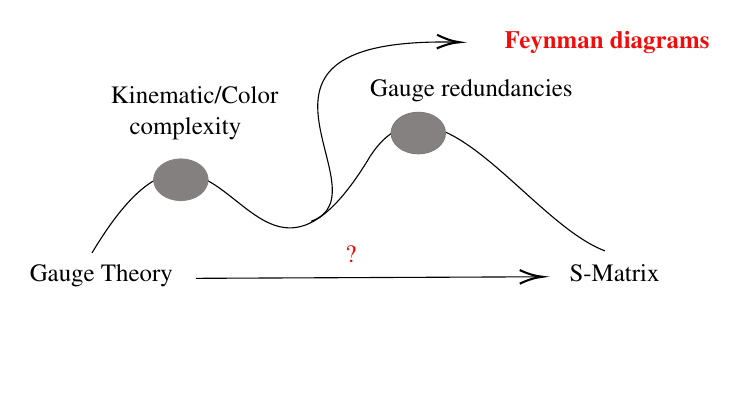
\begin{tikzpicture}[x=0.75pt,y=0.75pt,yscale=-1,xscale=1]
%uncomment if require: \path (0,300); %set diagram left start at 0, and has height of 300

%Curve Lines [id:da3663218891074064] 
\draw    (211.4,171.25) .. controls (275.46,64.25) and (285.26,224.75) .. (345.4,124.75) ;
%Shape: Ellipse [id:dp631421347808582] 
\draw  [color={rgb, 255:red, 134; green, 131; blue, 131 }  ,draw opacity=1 ][fill={rgb, 255:red, 133; green, 128; blue, 128 }  ,fill opacity=1 ] (241.14,136) .. controls (241.14,130.48) and (246.99,126) .. (254.21,126) .. controls (261.43,126) and (267.29,130.48) .. (267.29,136) .. controls (267.29,141.52) and (261.43,146) .. (254.21,146) .. controls (246.99,146) and (241.14,141.52) .. (241.14,136) -- cycle ;
%Curve Lines [id:da0018479507229188785] 
\draw    (345.4,124.75) .. controls (376.12,77.25) and (421.23,156.25) .. (458.49,170.25) ;
%Shape: Ellipse [id:dp37806345751603687] 
\draw  [color={rgb, 255:red, 128; green, 124; blue, 124 }  ,draw opacity=1 ][fill={rgb, 255:red, 133; green, 129; blue, 129 }  ,fill opacity=1 ] (355.53,113.5) .. controls (355.53,107.98) and (361.39,103.5) .. (368.61,103.5) .. controls (375.83,103.5) and (381.68,107.98) .. (381.68,113.5) .. controls (381.68,119.02) and (375.83,123.5) .. (368.61,123.5) .. controls (361.39,123.5) and (355.53,119.02) .. (355.53,113.5) -- cycle ;
%Straight Lines [id:da7438579232631651] 
\draw    (261.4,183.5) -- (426.42,182.76) ;
\draw [shift={(428.42,182.75)}, rotate = 179.74] [color={rgb, 255:red, 0; green, 0; blue, 0 }  ][line width=0.75]    (10.93,-3.29) .. controls (6.95,-1.4) and (3.31,-0.3) .. (0,0) .. controls (3.31,0.3) and (6.95,1.4) .. (10.93,3.29)   ;
%Curve Lines [id:da40606602539843883] 
\draw    (316.97,156) .. controls (355.02,142.32) and (265.25,67.01) .. (386.7,69.7) ;
\draw [shift={(388.54,69.75)}, rotate = 181.61] [color={rgb, 255:red, 0; green, 0; blue, 0 }  ][line width=0.75]    (10.93,-3.29) .. controls (6.95,-1.4) and (3.31,-0.3) .. (0,0) .. controls (3.31,0.3) and (6.95,1.4) .. (10.93,3.29)   ;

% Text Node
\draw (215.9,175.75) node [anchor=north] [inner sep=0.75pt]  [font=\small] [align=left] {{\fontfamily{ptm}\selectfont {\small  Gauge Theory}}\\{\fontfamily{ptm}\selectfont {\small  }}};
% Text Node
\draw (219.25,90) node [anchor=north west][inner sep=0.75pt]  [font=\small] [align=left] {{\small {\fontfamily{ptm}\selectfont Kinematic/Color}}\\{\small {\fontfamily{ptm}\selectfont  \ \ \ complexity}}};
% Text Node
\draw (344.1,86.5) node [anchor=north west][inner sep=0.75pt]  [font=\small] [align=left] {{\fontfamily{ptm}\selectfont {\small Gauge redundancies}}};
% Text Node
\draw (440.24,175.5) node [anchor=north west][inner sep=0.75pt]  [font=\small] [align=left] {{\fontfamily{ptm}\selectfont {\small S-Matrix}}};
% Text Node
\draw (332.23,166.5) node [anchor=north west][inner sep=0.75pt]  [font=\normalsize] [align=left] {{\fontfamily{ptm}\selectfont {\small \textcolor[rgb]{1,0,0}{?}}}};
% Text Node
\draw (408.97,63) node [anchor=north west][inner sep=0.75pt]  [font=\small] [align=left] {{\fontfamily{ptm}\selectfont {\small \textbf{\textcolor[rgb]{0.95,0.05,0.05}{Feynman diagrams}}}}};


\end{tikzpicture}
\end{center}
\vspace{-2.3em}
\tikzset{every picture/.style={line width=0.75pt}} %set default line width to 0.75pt        

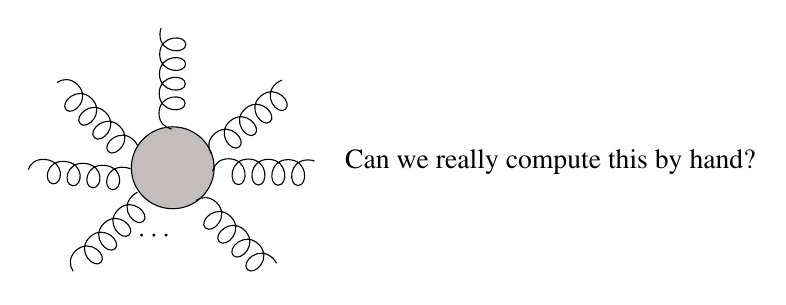
\begin{tikzpicture}[x=0.75pt,y=0.75pt,yscale=-1,xscale=1]
%uncomment if require: \path (0,300); %set diagram left start at 0, and has height of 300

%Shape: Spring [id:dp43786797179465176] 
\draw   (216.4,104.97) .. controls (219.03,103.2) and (222.94,102.68) .. (226.33,106.02) .. controls (233.1,112.72) and (224.24,121.49) .. (220.86,118.14) .. controls (217.47,114.8) and (226.33,106.02) .. (233.1,112.72) .. controls (239.87,119.41) and (231.01,128.19) .. (227.63,124.84) .. controls (224.24,121.49) and (233.1,112.72) .. (239.87,119.41) .. controls (246.64,126.11) and (237.78,134.88) .. (234.4,131.53) .. controls (231.01,128.19) and (239.87,119.41) .. (246.64,126.11) .. controls (253.41,132.8) and (244.56,141.58) .. (241.17,138.23) .. controls (237.78,134.88) and (246.64,126.11) .. (253.41,132.8) .. controls (254.2,133.59) and (254.78,134.4) .. (255.18,135.22) ;
%Shape: Ellipse [id:dp10564067273276767] 
\draw  [fill={rgb, 255:red, 196; green, 189; blue, 189 }  ,fill opacity=1 ] (252.25,146.07) .. controls (252.25,135.17) and (261.17,126.33) .. (272.19,126.33) .. controls (283.2,126.33) and (292.12,135.17) .. (292.12,146.07) .. controls (292.12,156.97) and (283.2,165.8) .. (272.19,165.8) .. controls (261.17,165.8) and (252.25,156.97) .. (252.25,146.07) -- cycle ;
%Shape: Spring [id:dp8051072896719512] 
\draw   (202.57,146.94) .. controls (203.45,144.19) and (206.11,141.62) .. (210.87,142.09) .. controls (220.4,143.03) and (219.26,154.27) .. (214.5,153.79) .. controls (209.74,153.32) and (210.87,142.09) .. (220.4,143.03) .. controls (229.92,143.98) and (228.78,155.21) .. (224.02,154.74) .. controls (219.26,154.27) and (220.4,143.03) .. (229.92,143.98) .. controls (239.44,144.92) and (238.31,156.15) .. (233.54,155.68) .. controls (228.78,155.21) and (229.92,143.98) .. (239.44,144.92) .. controls (248.97,145.87) and (247.83,157.1) .. (243.07,156.63) .. controls (238.31,156.15) and (239.44,144.92) .. (248.97,145.87) .. controls (250.08,145.98) and (251.05,146.23) .. (251.89,146.59) ;
%Shape: Spring [id:dp24229359788253813] 
\draw   (291.38,147.82) .. controls (292.02,144.73) and (294.46,141.66) .. (299.24,141.73) .. controls (308.81,141.87) and (308.63,154.27) .. (303.84,154.2) .. controls (299.06,154.13) and (299.24,141.73) .. (308.81,141.87) .. controls (318.38,142.01) and (318.2,154.41) .. (313.41,154.34) .. controls (308.63,154.27) and (308.81,141.87) .. (318.38,142.01) .. controls (327.95,142.15) and (327.77,154.55) .. (322.98,154.48) .. controls (318.2,154.41) and (318.38,142.01) .. (327.95,142.15) .. controls (337.52,142.28) and (337.34,154.69) .. (332.55,154.62) .. controls (327.77,154.55) and (327.95,142.15) .. (337.52,142.28) .. controls (338.64,142.3) and (339.63,142.49) .. (340.49,142.8) ;
%Shape: Spring [id:dp1840306550125722] 
\draw   (290.58,139.13) .. controls (289.05,136.36) and (288.91,132.46) .. (292.6,129.45) .. controls (299.99,123.43) and (307.96,133) .. (304.26,136.01) .. controls (300.57,139.02) and (292.6,129.45) .. (299.99,123.43) .. controls (307.38,117.41) and (315.35,126.98) .. (311.65,129.99) .. controls (307.96,133) and (299.99,123.43) .. (307.38,117.41) .. controls (314.77,111.38) and (322.73,120.96) .. (319.04,123.97) .. controls (315.35,126.98) and (307.38,117.41) .. (314.77,111.38) .. controls (322.16,105.36) and (330.12,114.94) .. (326.43,117.95) .. controls (322.73,120.96) and (314.77,111.38) .. (322.16,105.36) .. controls (323.02,104.66) and (323.9,104.17) .. (324.76,103.85) ;
%Shape: Spring [id:dp21851269782703253] 
\draw   (271.73,127.44) .. controls (268.6,126.81) and (265.5,124.41) .. (265.56,119.67) .. controls (265.68,110.2) and (278.2,110.35) .. (278.14,115.09) .. controls (278.08,119.82) and (265.56,119.67) .. (265.68,110.2) .. controls (265.79,100.73) and (278.32,100.88) .. (278.26,105.61) .. controls (278.2,110.35) and (265.68,110.2) .. (265.79,100.73) .. controls (265.91,91.25) and (278.44,91.4) .. (278.38,96.14) .. controls (278.32,100.88) and (265.79,100.73) .. (265.91,91.25) .. controls (266.03,81.78) and (278.55,81.93) .. (278.5,86.67) .. controls (278.44,91.4) and (265.91,91.25) .. (266.03,81.78) .. controls (266.04,80.67) and (266.23,79.69) .. (266.54,78.84) ;
%Shape: Spring [id:dp05024762380258474] 
\draw   (224.2,195.95) .. controls (222.44,193.32) and (221.96,189.44) .. (225.37,186.13) .. controls (232.21,179.5) and (240.98,188.36) .. (237.56,191.68) .. controls (234.14,194.99) and (225.37,186.13) .. (232.21,179.5) .. controls (239.05,172.87) and (247.82,181.73) .. (244.4,185.05) .. controls (240.98,188.36) and (232.21,179.5) .. (239.05,172.87) .. controls (245.88,166.24) and (254.65,175.1) .. (251.24,178.42) .. controls (247.82,181.73) and (239.05,172.87) .. (245.88,166.24) .. controls (252.72,159.61) and (261.49,168.47) .. (258.07,171.79) .. controls (254.65,175.1) and (245.88,166.24) .. (252.72,159.61) .. controls (253.52,158.83) and (254.35,158.27) .. (255.18,157.88) ;
%Shape: Spring [id:dp9217960437924791] 
\draw   (283.39,161.81) .. controls (286.03,160.03) and (289.94,159.51) .. (293.32,162.86) .. controls (300.09,169.56) and (291.24,178.33) .. (287.85,174.98) .. controls (284.47,171.64) and (293.32,162.86) .. (300.09,169.56) .. controls (306.86,176.25) and (298.01,185.03) .. (294.62,181.68) .. controls (291.24,178.33) and (300.09,169.56) .. (306.86,176.25) .. controls (313.63,182.95) and (304.78,191.72) .. (301.39,188.37) .. controls (298.01,185.03) and (306.86,176.25) .. (313.63,182.95) .. controls (320.4,189.64) and (311.55,198.42) .. (308.17,195.07) .. controls (304.78,191.72) and (313.63,182.95) .. (320.4,189.64) .. controls (321.2,190.43) and (321.78,191.24) .. (322.17,192.06) ;

% Text Node
\draw (254.1,174.78) node [anchor=north west][inner sep=0.75pt]    {$\cdots $};
% Text Node
\draw (354,136) node [anchor=north west][inner sep=0.75pt]   [align=left] {{\fontfamily{ptm}\selectfont Can we really compute this by hand?}};


\end{tikzpicture}

\end{frame}
\begin{frame}
    \frametitle{From Frynman diagram to On-shell method}
    The answer is On-shell method.
    \begin{center}
        

\tikzset{every picture/.style={line width=0.75pt}} %set default line width to 0.75pt        

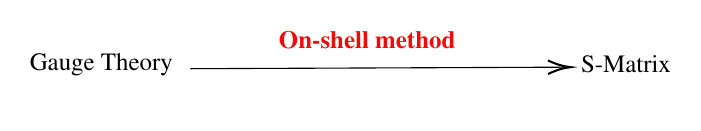
\begin{tikzpicture}[x=0.75pt,y=0.75pt,yscale=-1,xscale=1]
%uncomment if require: \path (0,300); %set diagram left start at 0, and has height of 300

%Straight Lines [id:da5445374886882226] 
\draw    (276.25,137) -- (457.5,136.26) ;
\draw [shift={(459.5,136.25)}, rotate = 179.77] [color={rgb, 255:red, 0; green, 0; blue, 0 }  ][line width=0.75]    (10.93,-3.29) .. controls (6.95,-1.4) and (3.31,-0.3) .. (0,0) .. controls (3.31,0.3) and (6.95,1.4) .. (10.93,3.29)   ;

% Text Node
\draw (233.4,128.25) node [anchor=north] [inner sep=0.75pt]  [font=\small] [align=left] {{\fontfamily{ptm}\selectfont {\small  Gauge Theory}}\\{\fontfamily{ptm}\selectfont {\small  }}};
% Text Node
\draw (463.24,129.5) node [anchor=north west][inner sep=0.75pt]  [font=\small] [align=left] {{\fontfamily{ptm}\selectfont {\small S-Matrix}}};
% Text Node
\draw (317.73,117.5) node [anchor=north west][inner sep=0.75pt]  [font=\normalsize] [align=left] {{\fontfamily{ptm}\selectfont {\small \textbf{\textcolor[rgb]{0.95,0.04,0.04}{On-shell method}}}}};


\end{tikzpicture}

    \end{center}

    On-shell here means that all quantities we use are gauge invariant and satisfy the on-shell condition.
    Specifically, there are many ingredients under this frame
    \begin{itemize}
        \item The analytic continuation for S-matrix.
        \item The color-ordered amplitudes.
        \item The BCFW recursion relation.
        \item The spinor helicity discription for amplitudes.
    \end{itemize}
\end{frame}
\section{Preliminary}
\begin{frame}
    \frametitle{A brief introduction to BCFW}
BCFW helps us solve one of the problems
\vspace{-1em}
\begin{figure}
    \centering
    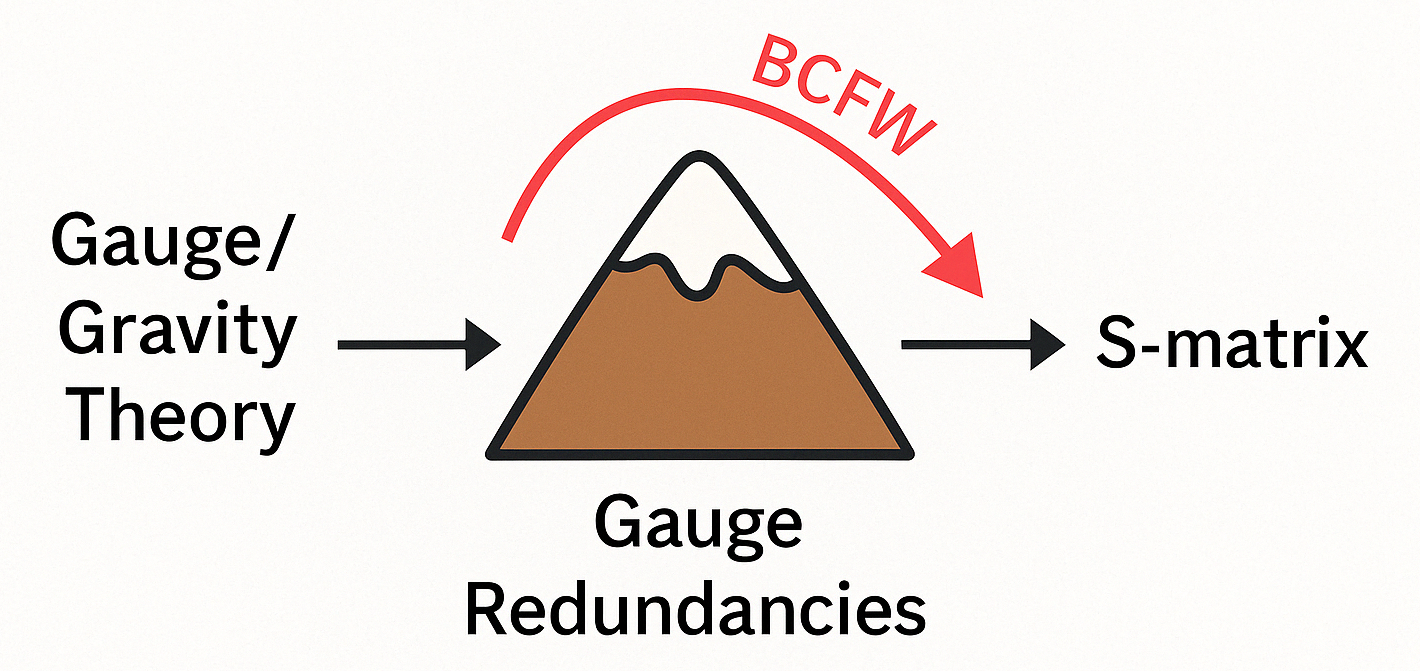
\includegraphics[width=0.5\textwidth]{BCFW.png}
\end{figure}
\vspace{-1em}
with the cost of introducing \textcolor{red}{complexed momentum}.

BCFW is a method to compute amplitudes recursively, proposed by 
\begin{itemize}
    \item Britto, Cachazo, Feng, arXiv: hep-th/0412308
    \item Britto, Cachazo, Feng, Witten, arXiv: hep-th/0501052

\end{itemize}
 


\begin{center}
    
 \tikzset{every picture/.style={line width=0.75pt}} %set default line width to 0.75pt        

 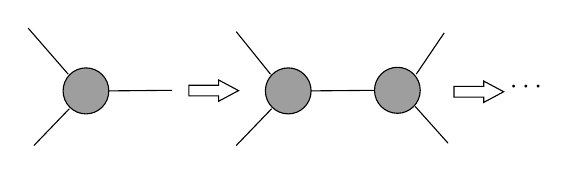
\begin{tikzpicture}[x=0.75pt,y=0.75pt,yscale=-1,xscale=1]
 %uncomment if require: \path (0,300); %set diagram left start at 0, and has height of 300
 
 %Shape: Ellipse [id:dp47704771803228196] 
 \draw  [fill={rgb, 255:red, 158; green, 158; blue, 158 }  ,fill opacity=1 ] (179.79,126.94) .. controls (179.79,120.82) and (184.73,115.86) .. (190.81,115.86) .. controls (196.89,115.86) and (201.82,120.82) .. (201.82,126.94) .. controls (201.82,133.06) and (196.89,138.02) .. (190.81,138.02) .. controls (184.73,138.02) and (179.79,133.06) .. (179.79,126.94) -- cycle ;
 %Straight Lines [id:da8859462256956995] 
 \draw    (163,96.75) -- (182.27,118.91) ;
 %Straight Lines [id:da980370255241411] 
 \draw    (201.82,126.94) -- (232.38,126.66) ;
 %Straight Lines [id:da41368612060172827] 
 \draw    (182.82,135.52) -- (165.75,153.25) ;
 %Right Arrow [id:dp6770308298589597] 
 \draw   (240.37,124.24) -- (254.74,124.24) -- (254.74,121.68) -- (264.32,126.8) -- (254.74,131.92) -- (254.74,129.36) -- (240.37,129.36) -- cycle ;
 %Shape: Ellipse [id:dp9789947232756657] 
 \draw  [fill={rgb, 255:red, 158; green, 158; blue, 158 }  ,fill opacity=1 ] (277.26,126.94) .. controls (277.26,120.82) and (282.19,115.86) .. (288.27,115.86) .. controls (294.35,115.86) and (299.28,120.82) .. (299.28,126.94) .. controls (299.28,133.06) and (294.35,138.02) .. (288.27,138.02) .. controls (282.19,138.02) and (277.26,133.06) .. (277.26,126.94) -- cycle ;
 %Straight Lines [id:da15853752019875] 
 \draw    (263.22,98.41) -- (279.74,118.91) ;
 %Straight Lines [id:da28595275955528565] 
 \draw    (299.28,126.94) -- (329.84,126.66) ;
 %Straight Lines [id:da7505788363123894] 
 \draw    (280.29,135.52) -- (263.22,153.25) ;
 %Shape: Ellipse [id:dp870376485686725] 
 \draw  [fill={rgb, 255:red, 158; green, 158; blue, 158 }  ,fill opacity=1 ] (351.87,126.66) .. controls (351.87,120.54) and (346.94,115.58) .. (340.86,115.58) .. controls (334.77,115.58) and (329.84,120.54) .. (329.84,126.66) .. controls (329.84,132.78) and (334.77,137.74) .. (340.86,137.74) .. controls (346.94,137.74) and (351.87,132.78) .. (351.87,126.66) -- cycle ;
 %Straight Lines [id:da5791423310908868] 
 \draw    (363.43,98.97) -- (349.94,118.91) ;
 %Straight Lines [id:da5454664407915119] 
 \draw    (349.43,134.42) -- (365.28,152.14) ;
 %Right Arrow [id:dp848095583389827] 
 \draw   (368.11,124.79) -- (382.49,124.79) -- (382.49,122.23) -- (392.07,127.35) -- (382.49,132.48) -- (382.49,129.92) -- (368.11,129.92) -- cycle ;
 
 % Text Node
 \draw (393.76,120.95) node [anchor=north west][inner sep=0.75pt]    {$\cdots $};
 
 
 \end{tikzpicture}
\end{center}

\end{frame}
\begin{frame}
    \frametitle{From real to complex -- Analytic Continuation}
    \textbf{Why can we conduct analytic continuation?}
\begin{itemize}
  \item Tree level scattering amplitudes are rational functions of Lorentz invariants, such as $\bm{p_{i\mu}p_j^\mu}$, $\bm{p_{i\mu}\epsilon_j^\mu}$.
  \item \textbf{Locality} tells us that any pole of a tree-level amplitude must correspond to a on-shell propagating particle. 
  \item There's only single pole, no branch cuts (logs, square roots, etc) at tree level.
\end{itemize}
    \begin{center}
    \tikz{
      \draw[double equal sign distance, -Implies, line width=1pt] (0,0) -- (0,-1.2);
    }
    \end{center}
\vspace{0.5em}
\centering
\textcolor{red}{Ampltudes can be shifted to complex plane}
\end{frame}

\begin{frame}
    \frametitle{Momentum Shift in BCFW}
    \textbf{What did BCFW do to make the shift?}

    Here we consider the case in which all particles are massless, $p_i^2 = 0$ for all $i = 1, 2, \dotsc, n$. We choose two momentum to be shifted oppositely 
    \begin{equation*}
        p_i\rightarrow\hat{p}_i(z)\equiv p_i-zk,\qquad p_j\rightarrow\hat{p}_j(z)\equiv p_j+zk
    \end{equation*}
    satisfying 
    \begin{equation*}
        k^2=0,\qquad p_i\cdot k=0,\qquad p_j\cdot k=0
    \end{equation*}

\begin{figure}
    \centering
    \begin{minipage}{0.45\textwidth}
        \tikzset{every picture/.style={line width=0.75pt}} %set default line width to 0.75pt        

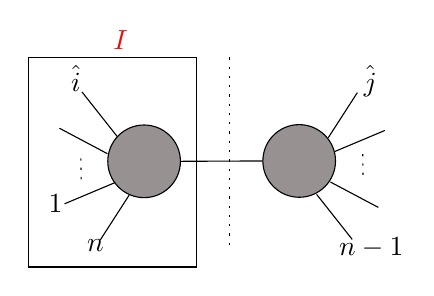
\begin{tikzpicture}[scale=0.7,x=0.75pt,y=0.75pt,yscale=-1,xscale=1]
%uncomment if require: \path (0,300); %set diagram left start at 0, and has height of 300

%Shape: Circle [id:dp47058391497271046] 
\draw  [fill={rgb, 255:red, 151; green, 145; blue, 145 }  ,fill opacity=1 ] (266.75,126) .. controls (266.75,112.19) and (277.94,101) .. (291.75,101) .. controls (305.56,101) and (316.75,112.19) .. (316.75,126) .. controls (316.75,139.81) and (305.56,151) .. (291.75,151) .. controls (277.94,151) and (266.75,139.81) .. (266.75,126) -- cycle ;
%Straight Lines [id:da8759716500759761] 
\draw    (249,78.25) -- (273.5,109.25) ;
%Straight Lines [id:da2121821831988906] 
\draw    (233.5,103.25) -- (266.5,120.75) ;
%Straight Lines [id:da6378763431676462] 
\draw  [dash pattern={on 0.84pt off 2.51pt}]  (350.75,54.38) -- (350.75,126.25) -- (350.75,187.63) ;
%Straight Lines [id:da7508961107891289] 
\draw  [dash pattern={on 0.84pt off 2.51pt}]  (248.25,124) -- (248.5,142.25) ;
%Straight Lines [id:da06317949320750826] 
\draw    (237,155.25) -- (271.5,140.75) ;
%Straight Lines [id:da403008866951158] 
\draw    (261.5,180.25) -- (281.5,149.25) ;
%Straight Lines [id:da8334043101335312] 
\draw    (423,119.25) -- (457.5,104.75) ;
%Straight Lines [id:da03451573841415356] 
\draw    (418.5,109.75) -- (438.5,78.75) ;
%Straight Lines [id:da025418352459996796] 
\draw    (420,140.25) -- (453,157.75) ;
%Straight Lines [id:da22879254297825424] 
\draw  [dash pattern={on 0.84pt off 2.51pt}]  (442.25,121) -- (442.5,139.25) ;
%Straight Lines [id:da2355772127149045] 
\draw    (410.5,148.75) -- (435,179.75) ;
%Shape: Rectangle [id:dp6752662310096104] 
\draw   (328,54.25) -- (328,198.75) -- (212,198.75) -- (212,54.25) -- cycle ;
%Straight Lines [id:da4580921639862495] 
\draw    (316.75,126) -- (373.5,125.75) ;
%Shape: Circle [id:dp8699671429684472] 
\draw  [fill={rgb, 255:red, 151; green, 145; blue, 145 }  ,fill opacity=1 ] (373.5,125.75) .. controls (373.5,111.94) and (384.69,100.75) .. (398.5,100.75) .. controls (412.31,100.75) and (423.5,111.94) .. (423.5,125.75) .. controls (423.5,139.56) and (412.31,150.75) .. (398.5,150.75) .. controls (384.69,150.75) and (373.5,139.56) .. (373.5,125.75) -- cycle ;

% Text Node
\draw (239.75,58.4) node [anchor=north west][inner sep=0.75pt]    {$\hat{i}$};
% Text Node
\draw (447.47,58.4) node [anchor=north] [inner sep=0.75pt]    {$\hat{j}$};
% Text Node
\draw (250.75,177.9) node [anchor=north west][inner sep=0.75pt]    {$n$};
% Text Node
\draw (224.25,147.4) node [anchor=north west][inner sep=0.75pt]    {$1$};
% Text Node
\draw (424.25,176.9) node [anchor=north west][inner sep=0.75pt]    {$n-1$};
% Text Node
\draw (268.75,34.4) node [anchor=north west][inner sep=0.75pt]  [color={rgb, 255:red, 241; green, 12; blue, 12 }  ,opacity=1 ]  {$I$};


\end{tikzpicture}
    \end{minipage}
    \hspace{1em}
    \begin{minipage}{0.45\textwidth}
        For a non-trival subset of generic momenta $\{p_i\}_{i\in I}$
    \begin{equation*}
        \hat{P}_I^2=P_I^2 -2zP_I\cdot k=-\frac{P_I^2}{z_I}(z-z_I) 
    \end{equation*}

    with $\textcolor{red}{\quad z_I=\frac{P_I^2}{2P_I\cdot k}}$.  
    \end{minipage}
\end{figure} 
\end{frame}

\begin{frame}
    \frametitle{Fantasitic result from Cauchy Theorem}
    %First, I will show the most important part in this report.
    \begin{block}{BCFW recursion relation}
        \begin{equation*}
            A_n=\sum_{\text{diagrams}\,I}\hat{A}_L(z_I)\frac{1}{P_I^2}\hat{A}_R(z_I)=\sum_{\text{diagrams}\,I}\raisebox{-1.3em}{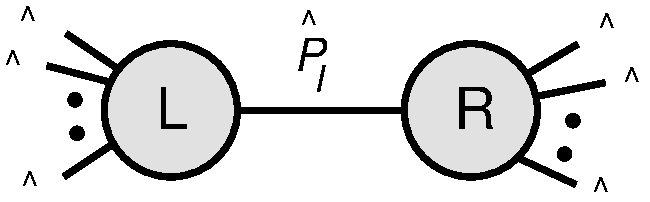
\includegraphics[height=3em]{recrel1.pdf}}
        \end{equation*}
    \end{block}
    Brief proof:
    
    We consider amplitude $A_n$ in terms of shifted momentum $\hat{p}_i^\mu$ instead of original real momentum. 
    \begin{equation*}
        A_n \longrightarrow \hat{A}_n(z)
    \end{equation*}
    
    If we consider the meromorphic function $\frac{\hat{A}_n(z)}{z}$ in the complex plane, pick a contour that surrounds the single pole at the origin. 
    \textcolor{red}{$\bigstar$ The most important point here is that}
    \begin{equation*}
        \boxed{\color{red}\mathrm{Res}|_{z=0}\frac{\hat{A}_n(z)}{z}=\hat{A}_n(0)=A_n}
    \end{equation*}
    It means that the original amplitude equals to the residue at origin.
\end{frame}
\begin{frame}
    From Cauchy Theorem, we can ontain
    \begin{equation*}
        A_n=-\sum_{z_I}\textrm{Res}|_{z=z_I}\frac{\hat{A}_n(z)}{z}+B_n,
    \end{equation*}
    where $B_n$ is the residue of the pole at $z=\infty$, called boundary term.
    \vspace{-1em}
    \begin{figure}[htbp]
        \centering
        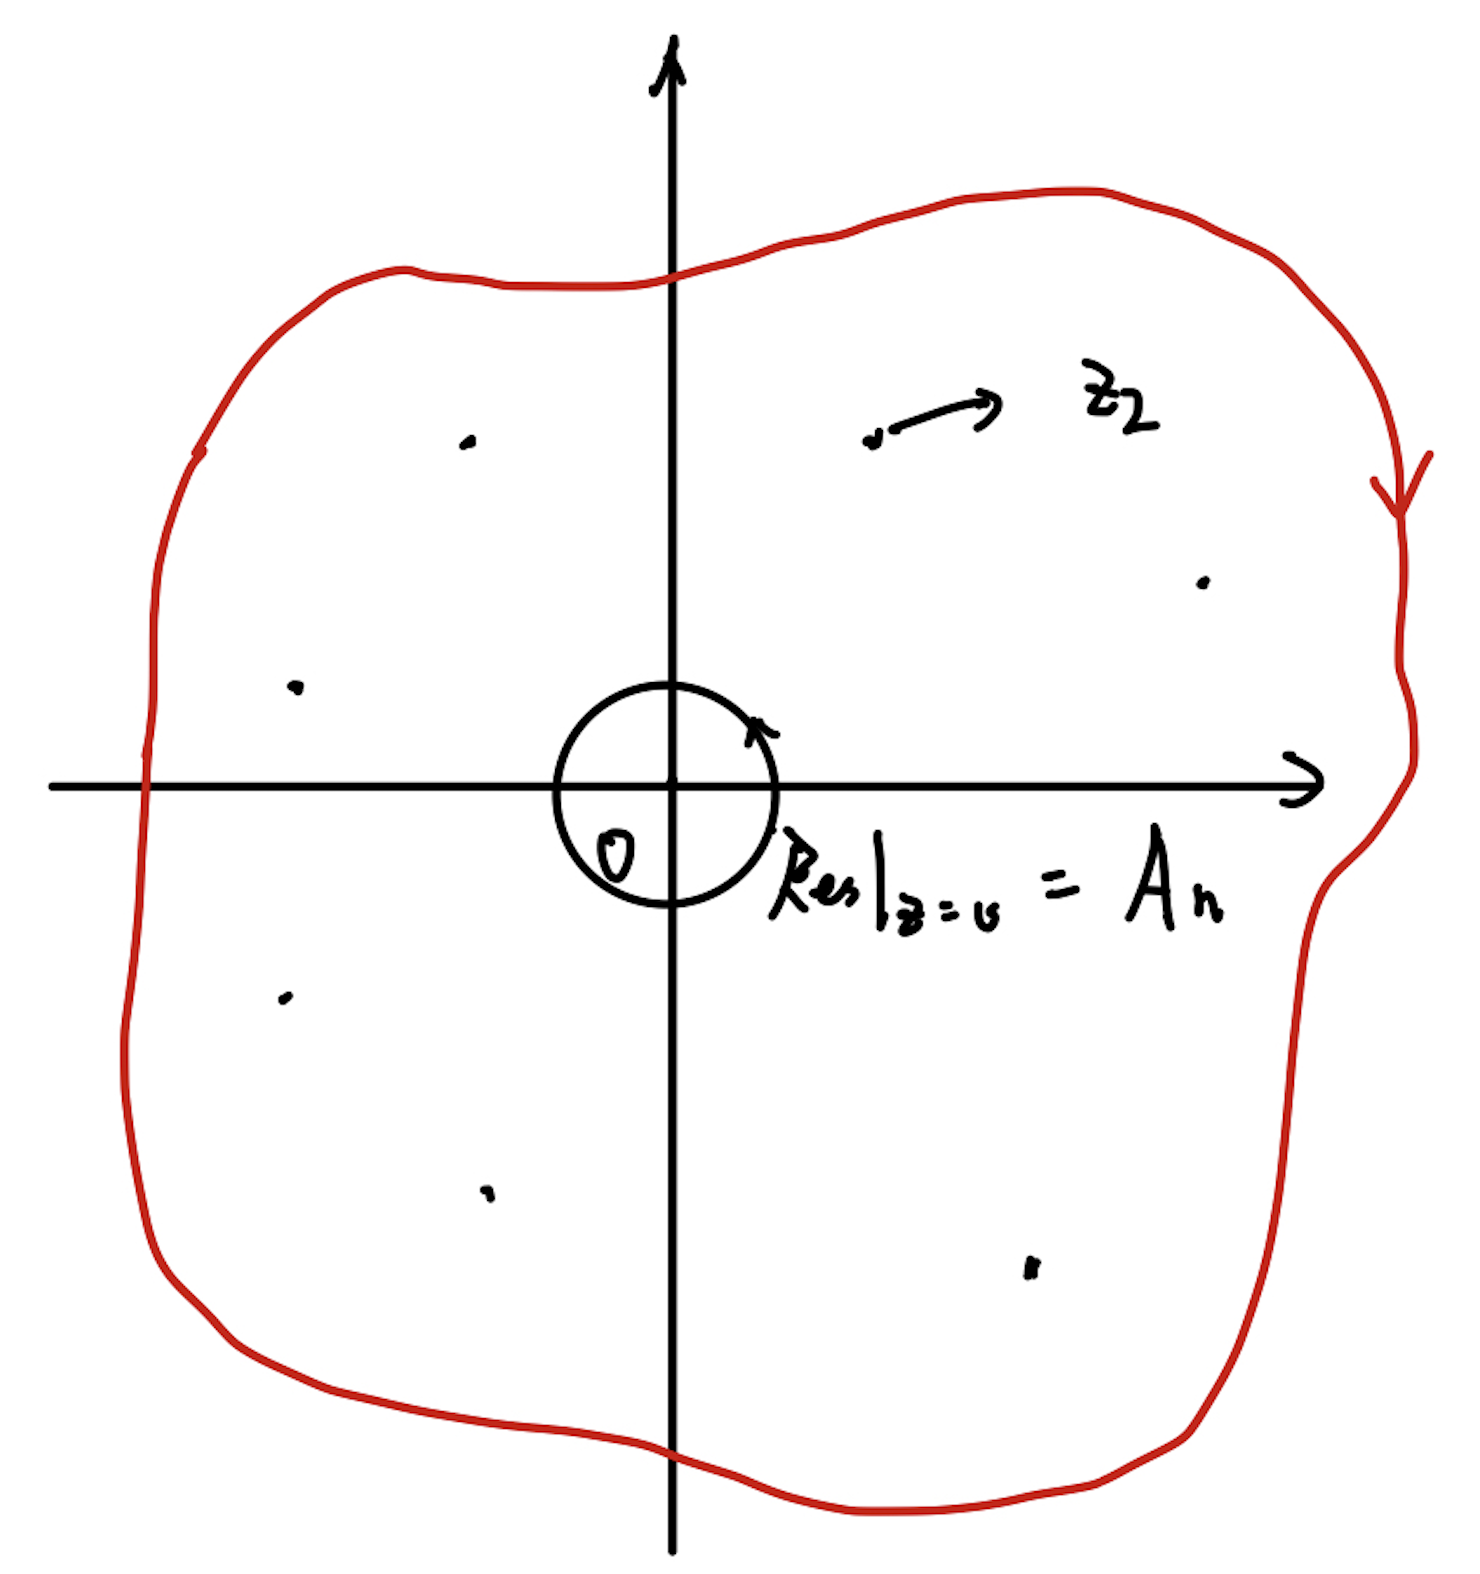
\includegraphics[width=0.3\textwidth]{CT.png}
    \end{figure}
    \vspace{-1.5em}
    %Then, at a $z_I$ pole, the propagator $\hat{P}_I^2$ goes to on-shell. In that limit, the shifted amplitude
    %\textcolor{red}{factorizes} into to on-shell parts (Unitarity)
    \begin{equation*}
        \hat{A}_n(z)\quad \xrightarrow{z\,\text{near}\,z_I} \quad \hat{A}_L(z_I)\frac{1}{\hat{P}_I^2}\hat{A}_R(z_I)= - \frac{z_I}{z-z_I}\hat{A}_L(z_I)\frac{1}{P_I^2}\hat{A}_R(z_I)
    \end{equation*}
    This makes it easy to evaluate the residue at $z=z_I$
    \begin{equation*}
        -\mathrm{Res}|_{z=z_I}\frac{\hat{A}_n(z)}{z}=\hat{A}_L(z_I)\frac{1}{P_I^2}\hat{A}_R(z_I)
    \end{equation*}
\end{frame}

\begin{frame}
    \frametitle{Large z behavior}
    In the BCFW formula, the boundary term $B_n$ affects a lot
    \begin{equation*}
        A_n=-\sum_{z_I}\mathrm{Res}|_{z=z_I}\frac{\hat{A}_n(z)}{z}+B_n,
    \end{equation*}
    In most applications. one assumes or much better, proves $B_n=0$. This is often justified by declaring a stronger condition
    \begin{equation*}
        \textcolor{red}{\hat{A}_n(z)\rightarrow 0 \quad \text{for} \quad z\rightarrow \infty} 
    \end{equation*}
    Here I show the large z behavior for gluon scattering 
    \begin{center}
        \begin{tabular}{lrc}
            \toprule
            $[i\, \textbackslash \, j\rangle $ & $+$ & $-$ \\
            \midrule
            $+$ & $1/z$ & $z^3$ \\
            $-$ & $1/z$ & $1/z$ \\
            \bottomrule
          \end{tabular}
    \end{center}
    
      
\end{frame}

\begin{frame}
    \frametitle{Spinor-Helicity formalisim}
In the part of introduction to BCFW
\begin{figure}
    \centering
    \begin{minipage}{0.45\textwidth}
        \centering
        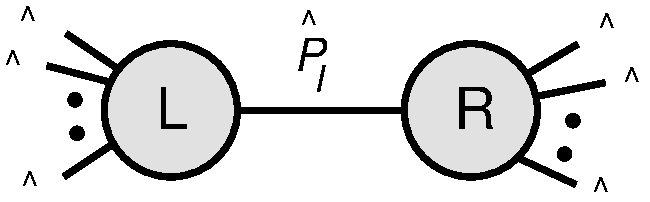
\includegraphics[height=4em]{recrel1.pdf} 
    \end{minipage}
    \hspace{0.01em}
    \begin{minipage}{0.45\textwidth}
        \centering
        \(
        \vcenter{\hbox{$\rightarrow$}} \quad \text{No helicity appears here}
        \)
    \end{minipage}
\end{figure}

but the S-matrix is a function of moentum $p_i$ and helicity $h_i$
\begin{center}
    
\tikzset{every picture/.style={line width=0.75pt}} %set default line width to 0.75pt        

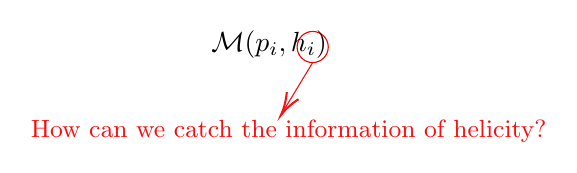
\begin{tikzpicture}[x=0.75pt,y=0.75pt,yscale=-1,xscale=1]
%uncomment if require: \path (0,300); %set diagram left start at 0, and has height of 300

%Shape: Circle [id:dp6973592945628315] 
\draw  [color={rgb, 255:red, 248; green, 0; blue, 0 }  ,draw opacity=1 ] (302.8,146.93) .. controls (302.81,142.78) and (306.18,139.44) .. (310.32,139.45) .. controls (314.47,139.46) and (317.81,142.83) .. (317.8,146.97) .. controls (317.79,151.11) and (314.42,154.46) .. (310.28,154.45) .. controls (306.14,154.44) and (302.79,151.07) .. (302.8,146.93) -- cycle ;
%Straight Lines [id:da7518027963985391] 
\draw [color={rgb, 255:red, 247; green, 18; blue, 18 }  ,draw opacity=1 ]   (310.28,154.45) -- (296.03,178.04) ;
\draw [shift={(295,179.75)}, rotate = 301.13] [color={rgb, 255:red, 247; green, 18; blue, 18 }  ,draw opacity=1 ][line width=0.75]    (10.93,-3.29) .. controls (6.95,-1.4) and (3.31,-0.3) .. (0,0) .. controls (3.31,0.3) and (6.95,1.4) .. (10.93,3.29)   ;

% Text Node
\draw (260.25,137.9) node [anchor=north west][inner sep=0.75pt]    {$\mathcal{M}( p_{i} ,h_{i})$};
% Text Node
\draw (173.25,181) node [anchor=north west][inner sep=0.75pt]  [font=\small,color={rgb, 255:red, 247; green, 13; blue, 13 }  ,opacity=1 ] [align=left] {How can we catch the information of helicity?};


\end{tikzpicture}
\end{center}
The answer is \textbf{Spinor-Helicity formalism} 
\(
\xrightarrow{\text{}} 
\)
Catch \(p_i\) and \(h_i\) at the same time.

\end{frame}
\begin{frame}
\frametitle{Spinor-helicity formalism}
    \begin{itemize}
        \item $\textbf{\text{Massless Case}}$\\
    \begin{equation*}
        p_\mu \sigma^\mu=p_{\alpha\dot{\alpha}}=\lambda_\alpha \tilde{\lambda}_{\dot{\alpha}}=\aket{\lambda}[\lambda|
    \end{equation*}
    There is an ambiguity for the definition, the momentum is invariant under the following redefinition
    \begin{equation*}
        \lambda \rightarrow t^{-1}\lambda, \qquad \tilde{\lambda}\rightarrow t\tilde{\lambda}, \qquad t\in\mathbb{C} 
    \end{equation*}
    same for
    \begin{equation*}
        \aket{\lambda}\rightarrow t^{-1}\aket{\lambda}, \qquad \sket{\lambda}\rightarrow t\sket{\lambda}
    \end{equation*}
    The scattering amplitudes should transform covariantly under little group scaling:
    \begin{equation*}
        \color{red} \mathcal{A}_n(\{\aket{1},\sket{1},h_1\},\ldots\{t_i^{-1}\aket{i},t_i\sket{i},h_i\},\ldots )=t_i^{2h_i}\mathcal{A}_n
    \end{equation*}
    \end{itemize}
\vspace{-2em}
    \begin{itemize}
    \item \textbf{Massive Case}\\
    It can also be handled in terms of spinor-helicity variable, see also 	arXiv:1709.04891 [hep-th] (Nima Arkani-Hamed, Tzu-Chen Huang, Yu-tin Huang).
    \end{itemize}
\end{frame}


\begin{frame}
    \frametitle{ On-shell 3-point can be completely determined}
    \textbf{On-shell 3-point for real momentum}

    Because of the constrain from momentum conservation and on-shell condition
    \begin{equation*}
        p_1=\kappa p_3, \qquad p_2=(1-\kappa)p_3 \quad(\text{Collinear})
    \end{equation*}
    All of the contribution 
    \begin{equation*}
        (p_1\cdot p_2),\quad (p_1\cdot p_3),\quad(p_2\cdot p_3)\quad =0  
    \end{equation*}
    In terms of Spinor- Helicity variable, we have 
    \begin{equation*}
        2p_1\cdot p_2=\avg{12}[21]=0\, \longrightarrow \,\avg{12}=[21]^*=0
    \end{equation*}
    \textcolor{red}{We can not obtain any thing nontrival from 3-point!}
    
    Of coure, you can introduce non-minimal interaction
    \begin{equation*}
        \mathcal{L}_3 \ni \frac{1}{\Lambda^2}\bar{\Psi}\slashed{D}(\Box \Psi)
    \end{equation*}
    but it still equals to 0 under the on-shell condition.
\end{frame}

\begin{frame}
    \textbf{Another necessarity to introduce complex momentum}

    If the momentum is complexed, we have 
    \begin{equation*}
        \avg{12}\neq[21]^*
    \end{equation*}
    Then we can obtain
    \begin{equation*}
        \aket{1}\propto \aket{2}\propto \aket{3} \qquad or \qquad \sket{1}\propto \sket{2}\propto \sket{3}
    \end{equation*}
    It means that 3-point amplitude depends only on angle brackets or squar brackets. Here I choose the first case to give an example
    \begin{equation*}
        A_3(1^{h_1},2^{h_2},3^{h_3})=c\avg{12}^{x_{12}}\avg{13}^{x_{13}}\avg{23}^{x_{23}},
    \end{equation*}
    Little group scaling tells us that
    \begin{equation*}
        t_1^{2h_1} A_3(1^{h_1},2^{h_2},3^{h_3})=ct_1^{-x_{12}}t_1^{-x_{13}}\avg{12}^{x_{12}}\avg{13}^{x_{13}}\avg{23}^{x_{23}}.
    \end{equation*}
    We can obtain
    \begin{equation*}
        2h_1=-x_{12}-x_{13}
    \end{equation*}
    Similarly, we can also obtain
    \begin{equation*}
        2h_2=-x_{12}-x_{23},\qquad 2h_3=-x_{13}-x_{23}.
    \end{equation*}
\end{frame}

\begin{frame}
    Then all index can be solved from this system of equations, so that
    \[
    \boxed{
    \begin{aligned}
        A_3^{h_1h_2h_3} &= c\avg{12}^{h_3-h_1-h_2}\avg{31}^{h_2-h_1-h_3}\avg{23}^{h_1-h_2-h_3}
        \quad & h_1+h_2+h_3 < 0 \\[0.5em]
        A_3^{h_1h_2h_3} &= c' [12]^{h_1+h_2-h_3}[23]^{h_2+h_3-h_1}[31]^{h_3+h_1-h_2}
        \quad & h_1+h_2+h_3 > 0
    \end{aligned}
        }
    \]

    \textbf{\textcolor{red}{$\star$\,All massless on-shell 3-point ampltides are completely determined by little group scaling!}}
    
    \textbf{Example}: 3-gluon amplitude\\
    \begin{equation*}
        A_3(g_1^-,g_2^-,g_3^+)=g\frac{\avg{12}^3}{\avg{23}\!\avg{31}}
    \end{equation*}
    There's another possibility 
    \begin{equation*}
        A_3(g_1^-,g_2^-,g_3^+)=g'\frac{[13][23]}{[12]^3}
    \end{equation*}
    but actually it comes from the \textcolor{red}{non-local} interaction $g'AA\frac{\partial}{\square}A$, so we discard it.
\end{frame}
\section{Introduction of quiver gauge theory}
\begin{frame}
    \frametitle{Introduction of Quiver or Moose gauge theory}
    \begin{figure}
        \centering
        \begin{minipage}{0.45\textwidth}
        Quiver: A container for carring arrows\\
        Moose: A kind of deer with large horns 
    \end{minipage}
    \begin{minipage}{0.45\textwidth}
        \centering
        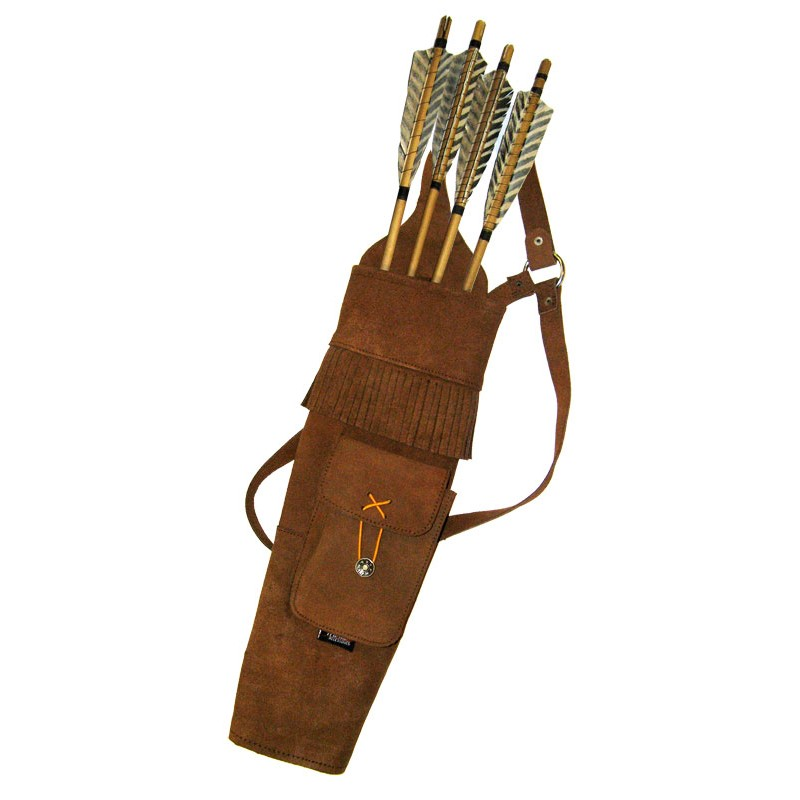
\includegraphics[width=0.3\linewidth]{Quiver.jpg}
        \hspace{1em}
        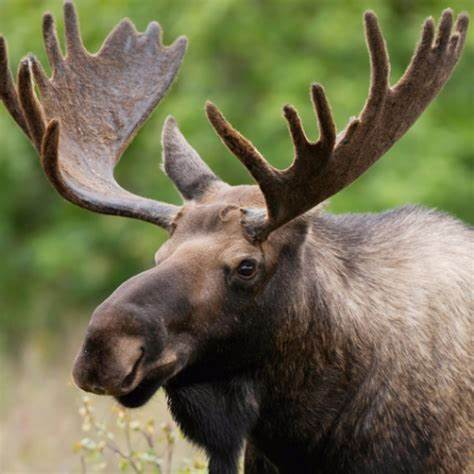
\includegraphics[width=0.3\textwidth]{Moose.jpeg}

    \end{minipage}
\end{figure}
    

    In the language of field theories, quiver gauge theories contain gauge fields and bi-fundamental scalars, summarized in a pictotial representaion.
    \begin{figure}
        \centering
        \begin{minipage}{0.45\textwidth}
            \centering
            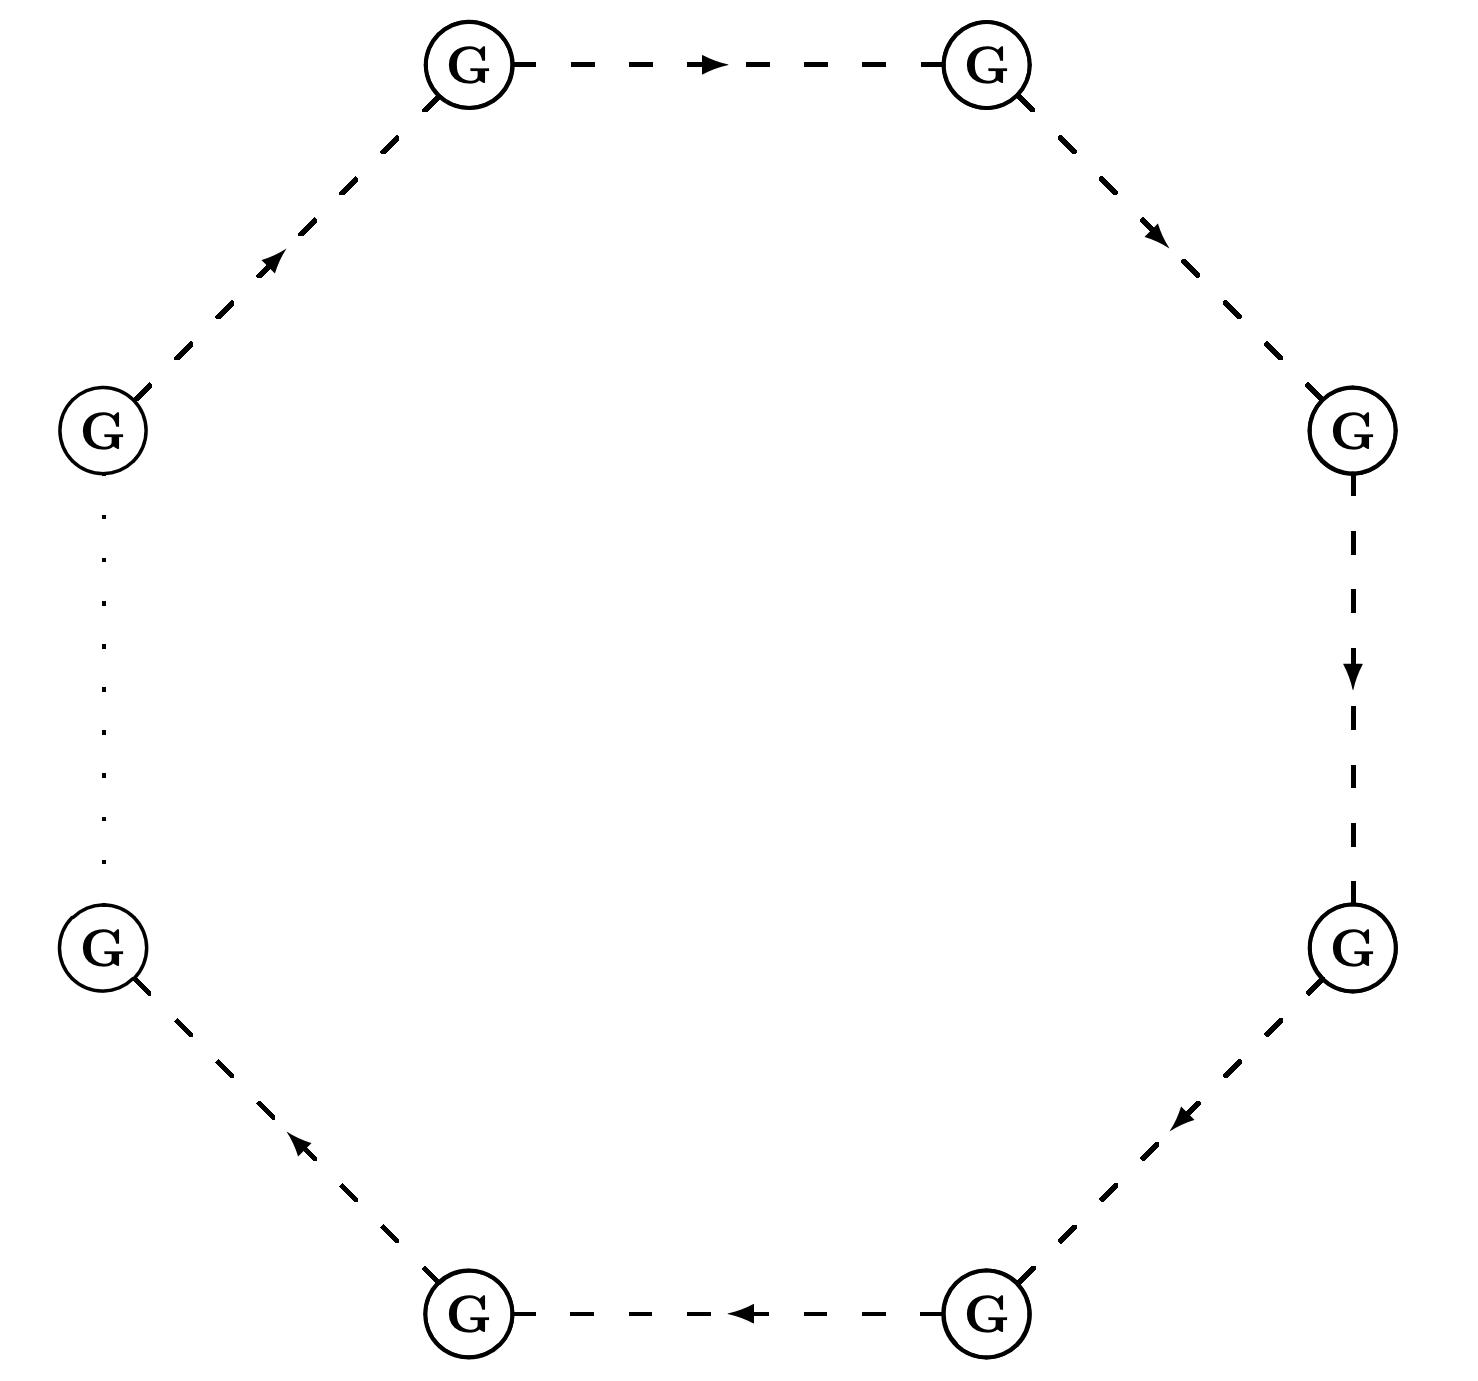
\includegraphics[width=0.6\textwidth]{Moosed.jpeg}
            \caption*{Moose diagram}
        \end{minipage}
        \hspace{1em}
        \begin{minipage}{0.3\textwidth}
            \begin{gather*}
                N\text{-sided polygon}\\
                G: \text{gauge group} \quad SU(m)\\
                \rightarrow : \text{Unitary scalar fields}\quad \Phi_{ij} 
            \end{gather*}
        \end{minipage}
        
    \end{figure}
\end{frame}
\begin{frame}
    \frametitle{Why we foucs on quiver gauge theory?}
    The lagrangian can be written like
    \begin{equation*}
        \mathcal{L}=-\sum_{i=1}^{N}\frac{1}{2}\mathrm{Tr}(F_i)^2+\sum_{i=1}^{N}\mathrm{Tr}[(D_\mu\Phi_i)^\dagger(D^\mu\Phi_i)],
    \end{equation*}
    here $F_i$ refers to the ith gauge field strength, scalar field $\Phi_i$ transformed under the \textcolor{red}{bi-fundamental} representation and the covariant derivative equals to
    \begin{equation*}
        D_\mu \Phi_i=\partial_\mu \Phi_i -ig_iA_{i\mu}\Phi_i+ig_{i+1}\Phi_i A_{i+1\mu}.
    \end{equation*}
    Here, gauge field and scalar field transformed like
    \begin{equation*}
        \bm{A_{i\mu}}\rightarrow U_i(x) \bm{A_{i\mu}} U_i^-(x)-\frac{i}{g_i}(\partial\mu U)U^{-1},\qquad \Phi_i\rightarrow U_i(x)\Phi_i U_{i+1}^-(x)
    \end{equation*}
    It is easy to confirm that this theory is invariant under $\prod_1^N SU(m)$ gauge group.
\end{frame}
\begin{frame}
    It has been proposed that this model actually discretized a five-dimension gauge theory with gauge group $SU(m)$, where 
    only the fifth dimension are latticed. So it is an effective theory for 5d gauge theory.
    \begin{itemize}
        \item If $SU(m)_1$ and $SU(m)_N$ are connected $\longrightarrow$ $S^2$ compactification
        \item If not connected $\longrightarrow$ $\mathrm{Interval}$ compactification
    \end{itemize}
    After higgsing the scalar field, we can obtain a spectrum
    \begin{equation*}
        M_k^2=4g^2f_s^2\sin^2\left(\frac{\pi k}{N}\right)
    \end{equation*}
    This is precisely the \textcolor{red}{Kaluza-Klein} spectrum under $S^2$ compactification. 
\end{frame}
\begin{frame}
    {What is relation to scattering amplitude?}
    The critical point is \textcolor{red}{locality}. 
    \begin{itemize}
        \item Space-Time Locality $\longrightarrow$ local field theories
        \item Theory Space Locality $\longrightarrow$ Discretized theory space
    \end{itemize}
    

\tikzset{every picture/.style={line width=0.75pt}} %set default line width to 0.75pt        
\begin{center}
    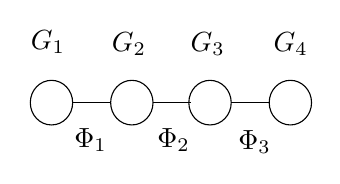
\begin{tikzpicture}[x=0.75pt,y=0.75pt,yscale=-1,xscale=1]
        %uncomment if require: \path (0,300); %set diagram left start at 0, and has height of 300
        
        %Shape: Ellipse [id:dp8504954329776364] 
        \draw   (104,129.25) .. controls (104,123.31) and (108.57,118.5) .. (114.2,118.5) .. controls (119.84,118.5) and (124.4,123.31) .. (124.4,129.25) .. controls (124.4,135.19) and (119.84,140) .. (114.2,140) .. controls (108.57,140) and (104,135.19) .. (104,129.25) -- cycle ;
        %Shape: Ellipse [id:dp885507200032482] 
        \draw   (219.1,129.25) .. controls (219.1,123.31) and (223.66,118.5) .. (229.3,118.5) .. controls (234.93,118.5) and (239.5,123.31) .. (239.5,129.25) .. controls (239.5,135.19) and (234.93,140) .. (229.3,140) .. controls (223.66,140) and (219.1,135.19) .. (219.1,129.25) -- cycle ;
        %Shape: Ellipse [id:dp7989991915217867] 
        \draw   (180.38,129.25) .. controls (180.38,123.31) and (184.95,118.5) .. (190.58,118.5) .. controls (196.22,118.5) and (200.79,123.31) .. (200.79,129.25) .. controls (200.79,135.19) and (196.22,140) .. (190.58,140) .. controls (184.95,140) and (180.38,135.19) .. (180.38,129.25) -- cycle ;
        %Shape: Ellipse [id:dp013562751387628191] 
        \draw   (142.71,129.25) .. controls (142.71,123.31) and (147.28,118.5) .. (152.92,118.5) .. controls (158.55,118.5) and (163.12,123.31) .. (163.12,129.25) .. controls (163.12,135.19) and (158.55,140) .. (152.92,140) .. controls (147.28,140) and (142.71,135.19) .. (142.71,129.25) -- cycle ;
        %Straight Lines [id:da15611587109210845] 
        \draw    (124.4,129.25) -- (142.71,129.25) ;
        %Straight Lines [id:da9794450917549196] 
        \draw    (163.12,129.25) -- (181.43,129.25) ;
        %Straight Lines [id:da4720621582644091] 
        \draw    (200.79,129.25) -- (219.1,129.25) ;
        
        % Text Node
        \draw (103,93.4) node [anchor=north west][inner sep=0.75pt]    {$G_{1}$};
        % Text Node
        \draw (142,94.4) node [anchor=north west][inner sep=0.75pt]    {$G_{2}$};
        % Text Node
        \draw (180,94.4) node [anchor=north west][inner sep=0.75pt]    {$G_{3}$};
        % Text Node
        \draw (220,94.4) node [anchor=north west][inner sep=0.75pt]    {$G_{4}$};
        % Text Node
        \draw (124,140.4) node [anchor=north west][inner sep=0.75pt]    {$\Phi _{1}$};
        % Text Node
        \draw (164,140.4) node [anchor=north west][inner sep=0.75pt]    {$\Phi _{2}$};
        % Text Node
        \draw (203,141.4) node [anchor=north west][inner sep=0.75pt]    {$\Phi _{3}$};
        \end{tikzpicture}
\end{center}
If we change this to a scattering diagram, and compute the large-z behavior
\begin{figure}
    \centering
\begin{minipage}{0.4\textwidth}


    \tikzset{every picture/.style={line width=0.75pt}} %set default line width to 0.75pt        

    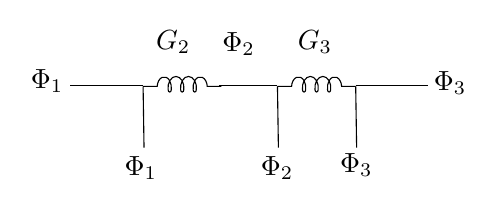
\begin{tikzpicture}[x=0.75pt,y=0.75pt,yscale=-1,xscale=1]
    %uncomment if require: \path (0,300); %set diagram left start at 0, and has height of 300
    
    %Shape: Inductor (Air Core) [id:dp932367781299785] 
    \draw   (274.98,130.32) -- (281.77,130.32) .. controls (281.87,128.3) and (282.81,126.57) .. (284.14,125.97) .. controls (285.47,125.36) and (286.92,126.01) .. (287.8,127.59) .. controls (288.47,128.82) and (288.75,130.41) .. (288.55,131.96) .. controls (288.55,132.56) and (288.21,133.05) .. (287.8,133.05) .. controls (287.38,133.05) and (287.04,132.56) .. (287.04,131.96) .. controls (286.85,130.41) and (287.12,128.82) .. (287.8,127.59) .. controls (288.58,126.27) and (289.67,125.53) .. (290.81,125.53) .. controls (291.95,125.53) and (293.05,126.27) .. (293.83,127.59) .. controls (294.5,128.82) and (294.78,130.41) .. (294.58,131.96) .. controls (294.58,132.56) and (294.24,133.05) .. (293.83,133.05) .. controls (293.41,133.05) and (293.07,132.56) .. (293.07,131.96) .. controls (292.88,130.41) and (293.16,128.82) .. (293.83,127.59) .. controls (294.61,126.27) and (295.7,125.53) .. (296.84,125.53) .. controls (297.99,125.53) and (299.08,126.27) .. (299.86,127.59) .. controls (300.53,128.82) and (300.81,130.41) .. (300.61,131.96) .. controls (300.61,132.56) and (300.28,133.05) .. (299.86,133.05) .. controls (299.44,133.05) and (299.11,132.56) .. (299.11,131.96) .. controls (298.91,130.41) and (299.19,128.82) .. (299.86,127.59) .. controls (300.73,126.01) and (302.18,125.36) .. (303.52,125.97) .. controls (304.85,126.57) and (305.79,128.3) .. (305.89,130.32) -- (312.67,130.32) ;
    %Straight Lines [id:da12934086227313735] 
    \draw    (239.95,129.92) -- (274.98,129.92) ;
    %Straight Lines [id:da483410968594159] 
    \draw    (274.98,130.32) -- (275.43,159.86) ;
    %Shape: Inductor (Air Core) [id:dp1480868197800882] 
    \draw   (339.72,130.32) -- (346.51,130.32) .. controls (346.6,128.3) and (347.55,126.57) .. (348.88,125.97) .. controls (350.21,125.36) and (351.66,126.01) .. (352.54,127.59) .. controls (353.21,128.82) and (353.48,130.41) .. (353.29,131.96) .. controls (353.29,132.56) and (352.95,133.05) .. (352.54,133.05) .. controls (352.12,133.05) and (351.78,132.56) .. (351.78,131.96) .. controls (351.59,130.41) and (351.86,128.82) .. (352.54,127.59) .. controls (353.32,126.27) and (354.41,125.53) .. (355.55,125.53) .. controls (356.69,125.53) and (357.78,126.27) .. (358.57,127.59) .. controls (359.24,128.82) and (359.52,130.41) .. (359.32,131.96) .. controls (359.32,132.56) and (358.98,133.05) .. (358.57,133.05) .. controls (358.15,133.05) and (357.81,132.56) .. (357.81,131.96) .. controls (357.62,130.41) and (357.89,128.82) .. (358.57,127.59) .. controls (359.35,126.27) and (360.44,125.53) .. (361.58,125.53) .. controls (362.72,125.53) and (363.81,126.27) .. (364.6,127.59) .. controls (365.27,128.82) and (365.55,130.41) .. (365.35,131.96) .. controls (365.35,132.56) and (365.01,133.05) .. (364.6,133.05) .. controls (364.18,133.05) and (363.84,132.56) .. (363.84,131.96) .. controls (363.65,130.41) and (363.92,128.82) .. (364.6,127.59) .. controls (365.47,126.01) and (366.92,125.36) .. (368.26,125.97) .. controls (369.59,126.57) and (370.53,128.3) .. (370.63,130.32) -- (377.41,130.32) ;
    %Straight Lines [id:da6722655237119544] 
    \draw    (311.79,129.92) -- (339.72,129.92) ;
    %Straight Lines [id:da3803917060459867] 
    \draw    (339.72,130.32) -- (340.17,159.86) ;
    %Straight Lines [id:da9202776931220129] 
    \draw    (377.41,130.32) -- (377.86,159.86) ;
    %Straight Lines [id:da09703581803647143] 
    \draw    (377.41,129.92) -- (412.44,129.92) ;
    
    % Text Node
    \draw (219.64,120.92) node [anchor=north west][inner sep=0.75pt]    {$\Phi _{1}$};
    % Text Node
    \draw (264.87,163) node [anchor=north west][inner sep=0.75pt]    {$\Phi _{1}$};
    % Text Node
    \draw (279.95,102.3) node [anchor=north west][inner sep=0.75pt]    {$G_{2}$};
    % Text Node
    \draw (311.87,103.11) node [anchor=north west][inner sep=0.75pt]    {$\Phi _{2}$};
    % Text Node
    \draw (330.5,163) node [anchor=north west][inner sep=0.75pt]    {$\Phi _{2}$};
    % Text Node
    \draw (348.23,102.3) node [anchor=north west][inner sep=0.75pt]    {$G_{3}$};
    % Text Node
    \draw (368.63,161.38) node [anchor=north west][inner sep=0.75pt]    {$\Phi _{3}$};
    % Text Node
    \draw (413.86,121.72) node [anchor=north west][inner sep=0.75pt]    {$\Phi _{3}$};
    
    
    \end{tikzpicture}
    
\end{minipage}
\hspace{1em}
\begin{minipage}{0.4\textwidth}
    \begin{equation*}
        \sim 1/z^{\textcolor{red}{\textcircled{\textcolor{black}{4}}}}
    \end{equation*}
\end{minipage}
\end{figure}
\end{frame}
\section{Scattering amplitudes from BCFW}
\begin{frame}
    \frametitle{Classification of Scattering Amplitudes}
    \centering
    For simplicity, we start from the two-site gauge theory with gauge fields $V_1$, $V_2$ and scalar fields $\Phi$, $\Phi^\dagger$. The amplitudes are classified by their multiplicity:
    
    \vspace{1em}

    \renewcommand{\arraystretch}{1.3}
    \setlength{\tabcolsep}{6pt}
    \begin{tabular}{|c|c|c|c|}
        \hline
        \textbf{3-point} & \textbf{4-point} & \textbf{5-point} & \textbf{6-point} \\
        \hline
        $\bm{V_1\Phi\Phi^\dagger}$ & $\bm{V_1V_1V_1V_1}$ & $\bm{V_1V_1V_1V_1V_1}$ & $\bm{V_1V_1V_1V_1V_1V_1}$ \\
        $\bm{V_2\Phi\Phi^\dagger}$ & $\bm{V_2V_2V_2V_2}$ & $\bm{V_2V_2V_2V_2V_2}$ & $\bm{V_2V_2V_2V_2V_2V_2}$ \\
        $\bm{V_1V_1V_1}$ & $\bm{\Phi^\dagger V_1V_1\Phi}$ & $\bm{\Phi^\dagger V_1V_1V_1\Phi}$ & $\bm{\Phi^\dagger V_1V_1V_1V_1\Phi}$ \\
        $\bm{V_2V_2V_2}$ & $\bm{\Phi V_2V_2\Phi^\dagger}$ & $\bm{\Phi V_2V_2V_2\Phi^\dagger}$ & $\bm{\Phi V_2V_2V_2V_2\Phi^\dagger}$ \\
        & $\bm{\Phi V_2 \Phi^\dagger V_1}$ & $\bm{V_2\Phi^\dagger V_1V_1\Phi}$ & $\bm{V_2V_2\Phi^\dagger V_1V_1\Phi}$ \\
        & $\bm{\Phi\Phi^\dagger\Phi\Phi^\dagger}$ & $\bm{\Phi V_2V_2\Phi^\dagger V_1}$ & $\bm{\Phi V_2V_2\Phi^\dagger V_1V_1}$ \\
        & & \textcolor{red}{$\Phi\Phi^\dagger\Phi\Phi^\dagger V_1$} & $\vdots$ \\
        & & \textcolor{red}{$\Phi\Phi^\dagger\Phi\Phi^\dagger V_2$} & $\vdots$ \\
        \hline
    \end{tabular}
\end{frame}
\begin{frame}
    \frametitle{Basic building block -- 3-point}
    From the previous section, we have known that there are only two kinds of 3 point amplitude
    \begin{gather*}
        A[1,2,3^+]=\frac{[23][31]}{[12]},\qquad A[1,2,3^-]=\frac{\avg{23}\!\avg{31}}{\avg{12}}\\
        A[3^+,4^+,5^-]=\frac{[34]^3}{[45][53]},\qquad A[3^-,4^-,5^+]=\frac{\avg{34}^3}{\avg{45}\!\avg{53}}
    \end{gather*}
    By using the 3 point building block, we can construct 4 point color-ordered amplitudes from BCFW recursion relation.
\end{frame}
\begin{frame}
    \frametitle{Gauge boson sector}
    \begin{itemize}
        \item n$ V_1$ or n$V_2$\\
        This part is completely the same as the pure gluon amplitude, so we can directly borrow the
        existing results.
        \begin{equation*}
            \boxed{\text{Parke - Talyor Formula}:\quad A[\cdots,i^-,\cdots,j^-,\cdots]=\frac{\avg{ij}^4}{\avg{12}\!\avg{23}\cdots\avg{n1}}}
        \end{equation*}
        \textcolor{red}{Notice that this formula only applies to MHV amplitudes, although the NMHV can be completely solved.}
    \end{itemize}
\end{frame}

\begin{frame}
    \frametitle{SQCD like sector}
    \begin{itemize}
        \item $\Phi^\dagger V_1V_1\Phi$\\
        Here we compute the color-ordered amplitude $A[1,2,3^+,4^-]$. We choose $[2,3\rangle$ shift
        \begin{gather*}
        \hat{\sket{2}}=\sket{2}-z\sket{3},\qquad \hat{\aket{2}}=\aket{2} \\
        \hat{\sket{3}}=\sket{3},\qquad \hat{\aket{3}}=\aket{3}+z\aket{2}
        \end{gather*}
        The amplitudes can be computed 
        \begin{align*}
            A[1,2,3^+,4^-]=(-1)\frac{\avg{14}^2\avg{24}^2}{\mdavg{12}{23}\!\mdavg{34}{41}}
        \end{align*}
        \item $\Phi^\dagger V_1V_1V_1\Phi$
            \begin{equation*}
                A[1,2,3^+,4^+,5^-]=\frac{\avg{15}^2\!\avg{25}^2}{\mdavg{12}{23}\!\mdavg{34}{45}\!\avg{51}}
            \end{equation*}
    \end{itemize}
\end{frame}

\begin{frame}
    \begin{itemize}
        \item $\Phi^\dagger (nV_1)\Phi$
            \begin{equation*}
                A[1,2,\cdots,(n+2)^-]=(-1)^{n+1}\frac{\avg{1,n+2}^2\avg{2,n+2}^2}{\mdavg{12}{23}\cdots\mdavg{n+1,n+2}{n+2,1}}
            \end{equation*}
            \textcolor{red}{$\star$ Bonus relation: \begin{equation*}
                A[1,2,3^+,4^+]=0\quad \Rightarrow  \quad A[1,2,3^+,\cdots,n^+]=0 \end{equation*}}
        For the amplitude $\Phi (nV_2)\Phi^\dagger$, we can obtain nearly the same expression.
    \end{itemize}
\end{frame}

\begin{frame}
    \frametitle{Pure 2-site amplitude}
    \begin{itemize}
        \item $\Phi V_2 \Phi^\dagger V_1$
        \begin{equation*}
            A[1,2,3_1^+,4_2^-]=\frac{\mdavg{14}{24}}{\mdavg{13}{23}}
        \end{equation*}
        \item $\Phi V_2 \Phi^\dagger V_1V_1$
        \begin{equation*}
            A[1,2,3_1^+,4_1^+,5_2^-]=(-1)\frac{\avg{2\textcolor{green}{5}}^2\!\avg{1\textcolor{green}{5}}^2}{\textcolor{blue}{\mdavg{23}{34}\!\avg{41}}\textcolor{red}{\mdavg{25}{51}}}
        \end{equation*}
        \item $\Phi V_2V_2 \Phi^\dagger V_1V_1$
        \begin{equation*}
            A[1,2,3_1^+,4_1^+,5_2^+,6_2^-]=\frac{\avg{2\textcolor{green}{6}}^2\!\avg{1\textcolor{green}{6}}^2}{\textcolor{blue}{\mdavg{23}{34}\!\avg{41}}\!\textcolor{red}{\mdavg{25}{56}\!\avg{61}}}
        \end{equation*}       
    \end{itemize}
\end{frame}

\begin{frame}
    \begin{itemize}
        \item Compact formula for general case
        \begin{equation*}
            A=\frac{\asqu{2\textcolor{green}{a}}\!\asqu{1\textcolor{green}{a}}}{\underbrace{\avg{2\textcolor{blue}{\star}}\cdots \avg{\textcolor{blue}{\star}1}}_{SU(N_1)}\underbrace{\avg{2\textcolor{red}{\ast} }\cdots \avg{\textcolor{red}{\ast} 1}}_{SU(N_2)}}
        \end{equation*} 
        \begin{minipage}{0.7\textwidth}
            \raggedright  % 或者 \centering 或 \raggedleft
            \textcolor{green}{Green:} \,Particle with $-$ helicity\\
            \textcolor{blue}{Blue:}\, Particle belongs to the first gauge group\\
            \textcolor{red}{Red:}\, Particle belongs to the second gauge group\\
            $\star$: \,Order for gauge group 1\\
            $\ast$: \,Order for gauge group 2 
            \end{minipage}
       
    \end{itemize}
\end{frame}
\section{Summary and Outlook}
\begin{frame}
    \frametitle{Summary}
    \begin{itemize}
        \item Introduce the on-shell method, including BCFW recursion relation, color-ordered amplitudes. etc.
        \item Introduce a (de)constructed gauge theory model, which is an effective field theory for 5 dimension gauge theory.
        \item The locality plays an important role to relate the spacetime locality and field space locality.
        \item Much of the scattering amplitudes in this model can be recursively computed by BCFW, and some compact formulas are offered.
    \end{itemize}
\end{frame}
\begin{frame}
    \frametitle{Possible future work}

\begin{center}
\tikzset{every picture/.style={line width=0.75pt}} %set default line width to 0.75pt        

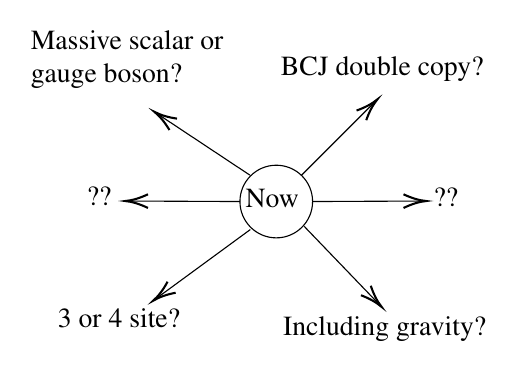
\begin{tikzpicture}[x=0.75pt,y=0.75pt,yscale=-1,xscale=1]
%uncomment if require: \path (0,300); %set diagram left start at 0, and has height of 300

%Shape: Circle [id:dp9858548351804828] 
\draw   (351.75,140.5) .. controls (351.75,130.84) and (359.59,123) .. (369.25,123) .. controls (378.91,123) and (386.75,130.84) .. (386.75,140.5) .. controls (386.75,150.16) and (378.91,158) .. (369.25,158) .. controls (359.59,158) and (351.75,150.16) .. (351.75,140.5) -- cycle ;
%Straight Lines [id:da97880204376832] 
\draw    (382.75,152.5) -- (418.61,189.81) ;
\draw [shift={(420,191.25)}, rotate = 226.13] [color={rgb, 255:red, 0; green, 0; blue, 0 }  ][line width=0.75]    (10.93,-3.29) .. controls (6.95,-1.4) and (3.31,-0.3) .. (0,0) .. controls (3.31,0.3) and (6.95,1.4) .. (10.93,3.29)   ;
%Straight Lines [id:da40380915410006823] 
\draw    (381.25,128) -- (416.59,92.66) ;
\draw [shift={(418,91.25)}, rotate = 135] [color={rgb, 255:red, 0; green, 0; blue, 0 }  ][line width=0.75]    (10.93,-3.29) .. controls (6.95,-1.4) and (3.31,-0.3) .. (0,0) .. controls (3.31,0.3) and (6.95,1.4) .. (10.93,3.29)   ;
%Straight Lines [id:da3536680968554168] 
\draw    (356.5,127.75) -- (312.17,98.36) ;
\draw [shift={(310.5,97.25)}, rotate = 33.55] [color={rgb, 255:red, 0; green, 0; blue, 0 }  ][line width=0.75]    (10.93,-3.29) .. controls (6.95,-1.4) and (3.31,-0.3) .. (0,0) .. controls (3.31,0.3) and (6.95,1.4) .. (10.93,3.29)   ;
%Straight Lines [id:da43484293892230164] 
\draw    (356.75,154) -- (311.61,187.07) ;
\draw [shift={(310,188.25)}, rotate = 323.77] [color={rgb, 255:red, 0; green, 0; blue, 0 }  ][line width=0.75]    (10.93,-3.29) .. controls (6.95,-1.4) and (3.31,-0.3) .. (0,0) .. controls (3.31,0.3) and (6.95,1.4) .. (10.93,3.29)   ;
%Straight Lines [id:da7682811881365084] 
\draw    (351.75,140.5) -- (298.5,140.26) ;
\draw [shift={(296.5,140.25)}, rotate = 0.26] [color={rgb, 255:red, 0; green, 0; blue, 0 }  ][line width=0.75]    (10.93,-3.29) .. controls (6.95,-1.4) and (3.31,-0.3) .. (0,0) .. controls (3.31,0.3) and (6.95,1.4) .. (10.93,3.29)   ;
%Straight Lines [id:da38096838344174566] 
\draw    (386.75,140.5) -- (439.5,140.26) ;
\draw [shift={(441.5,140.25)}, rotate = 179.74] [color={rgb, 255:red, 0; green, 0; blue, 0 }  ][line width=0.75]    (10.93,-3.29) .. controls (6.95,-1.4) and (3.31,-0.3) .. (0,0) .. controls (3.31,0.3) and (6.95,1.4) .. (10.93,3.29)   ;

% Text Node
\draw (353.25,133) node [anchor=north west][inner sep=0.75pt]   [align=left] {{\fontfamily{ptm}\selectfont Now}};
% Text Node
\draw (371.25,194.5) node [anchor=north west][inner sep=0.75pt]   [align=left] {{\fontfamily{ptm}\selectfont Including gravity?}};
% Text Node
\draw (370.25,69.5) node [anchor=north west][inner sep=0.75pt]   [align=left] {{\fontfamily{ptm}\selectfont BCJ double copy?}};
% Text Node
\draw (249.75,57) node [anchor=north west][inner sep=0.75pt]   [align=left] {{\fontfamily{ptm}\selectfont Massive scalar or}\\{\fontfamily{ptm}\selectfont  gauge boson?}};
% Text Node
\draw (262.75,191) node [anchor=north west][inner sep=0.75pt]   [align=left] {{\fontfamily{ptm}\selectfont 3 or 4 site?}};
% Text Node
\draw (276.75,132) node [anchor=north west][inner sep=0.75pt]   [align=left] {{\fontfamily{ptm}\selectfont ??}};
% Text Node
\draw (443.75,132.5) node [anchor=north west][inner sep=0.75pt]   [align=left] {{\fontfamily{ptm}\selectfont ??}};


\end{tikzpicture}
\end{center}
\end{frame}
\begin{frame}
    \centering
    \Huge Thanks for your attention!
\end{frame}
\appendix
\section{Appendix}
\begin{frame}
    \frametitle{Color structure}
    \begin{itemize}
        \item n$ V_1$ or n$V_2$\\
        This part is completely the same as the pure gluon amplitude, so we can directly borrow the
        existing results.
        \begin{equation*}
            \boxed{\text{Parke - Talyor Formula}:\quad A[\cdots,i^-,\cdots,j^-,\cdots]=\frac{\avg{ij}^4}{\avg{12}\!\avg{23}\cdots\avg{n1}}}
        \end{equation*}
        \textcolor{red}{Notice that this formula only applies for MHV amplitudes, although the NMHV can be completely solved.}
    \end{itemize}
\end{frame}

\begin{frame}
    \begin{itemize}
        \item $\Phi^\dagger V_1V_1\Phi$
        \begin{figure}
            \centering
            \begin{subfigure}{0.3\textwidth}
              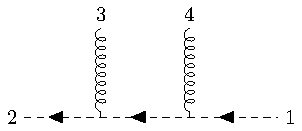
\includegraphics[width=\linewidth]{sch.pdf}
              \caption{s channel}
            \end{subfigure}
            \hfill
            \begin{subfigure}{0.3\textwidth}
              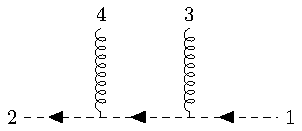
\includegraphics[width=\linewidth]{uch.pdf}
              \caption{u channel}
            \end{subfigure}
            \hfill
            \begin{subfigure}{0.3\textwidth}
              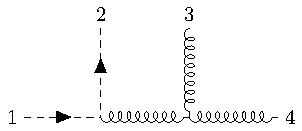
\includegraphics[width=\linewidth]{tch.pdf}
              \caption{t channel}
            \end{subfigure}
          \end{figure}
        The color factor can be written respectively as following
        \begin{equation*}
            r_s=\mathrm{Tr}[\Phi_2^\dagger T^{a_3}T^{a_4}\Phi_1],\,r_u=\mathrm{Tr}[\Phi_2^\dagger T^{a_4}T^{a_3}\Phi_1],\,
            r_t=\mathrm{Tr}[\Phi_2^\dagger [T^{a_3},T^{a_4}]\Phi_1]
        \end{equation*}
        We can easily obtain a similar Jacobbi relation
        \begin{equation*}
            r_t=r_s-r_u
        \end{equation*}
        Then we can accomplish the color decomposition and define the corressponding color-ordered amplitudes.
    \end{itemize}
\end{frame}

\begin{frame}
    \begin{itemize}
        \item[] For example, in the 4pt. case, the full amplitude can be decomposed to the following form
        \begin{align*}
            \mathcal{A}_4(\Phi^\dagger V_1V_1\Phi)&=A_s r_s+A_u r_u+A_t r_t\\
            &=A_s r_s+A_u r_u+A_t(r_s-r_u)\\
            &=(A_s+A_t)r_s+(A_u-A_t)r_u
        \end{align*}
        The two subamplitudes can be defined as color-ordered amplitude with order \textcolor{red}{[1,2,3,4]} and 
        \textcolor{red}{[1,2,4,3]} respectively.

        \vspace{0.5em}
        Of course, for the type $\Phi^\dagger(nV_1)\Phi$ and $\Phi (nV_2) \Phi^\dagger$, we can do the same thing to define the color-ordered amplitudes.
        It should be noticed that the order only has the relation with the order of external gluon line.
        \begin{equation*}
            [1,2,\sigma(3),\sigma(4),\cdots,\sigma(n)]
        \end{equation*}
    \end{itemize}
\end{frame}

\begin{frame}
    \begin{itemize}
        \item $\Phi V_2 \Phi^\dagger V_1$\\
        The color structure for this kind of amplitude has special form, like
        \begin{equation*}
            (T_1^a)_{ij}(T_2^b)_{\bar{j}\bar{i}}
        \end{equation*}
        It is more straightforward to observe the color structure in terms of double line notation as follows 
        \vspace{0.5em}

        \tikzset{every picture/.style={line width=0.75pt}} %set default line width to 0.75pt        

        \begin{tikzpicture}[x=0.75pt,y=0.75pt,yscale=-1,xscale=1]
%uncomment if require: \path (0,300); %set diagram left start at 0, and has height of 300

%Straight Lines [id:da7604191870446242] 
\draw [color={rgb, 255:red, 255; green, 0; blue, 0 }  ,draw opacity=1 ]   (100,100) -- (150,100) ;
%Straight Lines [id:da7895005569652712] 
\draw [color={rgb, 255:red, 0; green, 110; blue, 237 }  ,draw opacity=1 ]   (100,110) -- (190,110) ;
%Straight Lines [id:da19217218880843812] 
\draw [color={rgb, 255:red, 255; green, 0; blue, 0 }  ,draw opacity=1 ]   (150,50) -- (150,100) ;
%Straight Lines [id:da7866299736623521] 
\draw [color={rgb, 255:red, 255; green, 0; blue, 0 }  ,draw opacity=1 ]   (160,50) -- (160,100) ;
%Straight Lines [id:da5667542352395977] 
\draw [color={rgb, 255:red, 0; green, 118; blue, 255 }  ,draw opacity=1 ]   (190,110) -- (190,160) ;
%Straight Lines [id:da33701635654582174] 
\draw [color={rgb, 255:red, 0; green, 118; blue, 255 }  ,draw opacity=1 ]   (200,110) -- (200,160) ;
%Straight Lines [id:da7076492571881566] 
\draw [color={rgb, 255:red, 255; green, 0; blue, 0 }  ,draw opacity=1 ]   (299,100) -- (389,100) ;
%Straight Lines [id:da3803886589182971] 
\draw [color={rgb, 255:red, 0; green, 113; blue, 255 }  ,draw opacity=1 ]   (200,110) -- (250,110) ;
\draw  [color={rgb, 255:red, 255; green, 4; blue, 37 }  ,draw opacity=1 ] (128,103.83) -- (120,100.45) -- (127.97,96.99) ;
\draw  [color={rgb, 255:red, 255; green, 4; blue, 37 }  ,draw opacity=1 ] (153.28,70.33) -- (150.12,78.42) -- (146.44,70.55) ;
\draw  [color={rgb, 255:red, 255; green, 4; blue, 37 }  ,draw opacity=1 ] (156.49,77.35) -- (160.07,69.44) -- (163.33,77.49) ;
\draw  [color={rgb, 255:red, 255; green, 4; blue, 37 }  ,draw opacity=1 ] (340,102.83) -- (332,99.45) -- (339.97,95.99) ;
\draw  [color={rgb, 255:red, 0; green, 119; blue, 255 }  ,draw opacity=1 ] (120.93,107.08) -- (128.98,110.35) -- (121.06,113.93) ;
\draw  [color={rgb, 255:red, 0; green, 119; blue, 255 }  ,draw opacity=1 ] (193.4,129.42) -- (190,137.42) -- (186.55,129.45) ;
\draw  [color={rgb, 255:red, 0; green, 119; blue, 255 }  ,draw opacity=1 ] (196.55,138.41) -- (200,130.44) -- (203.4,138.44) ;
\draw  [color={rgb, 255:red, 0; green, 119; blue, 255 }  ,draw opacity=1 ] (220.93,107.08) -- (228.98,110.35) -- (221.06,113.93) ;
%Straight Lines [id:da696489944746132] 
\draw [color={rgb, 255:red, 0; green, 113; blue, 255 }  ,draw opacity=1 ]   (300,110) -- (350,110) ;
\draw  [color={rgb, 255:red, 0; green, 119; blue, 255 }  ,draw opacity=1 ] (321,107) -- (329.05,110.27) -- (321.13,113.84) ;
%Straight Lines [id:da24340791537710427] 
\draw [color={rgb, 255:red, 0; green, 118; blue, 255 }  ,draw opacity=1 ]   (350,110) -- (350,160) ;
\draw  [color={rgb, 255:red, 0; green, 119; blue, 255 }  ,draw opacity=1 ] (353.4,129.42) -- (350,137.42) -- (346.55,129.45) ;
%Straight Lines [id:da7298898466192736] 
\draw [color={rgb, 255:red, 0; green, 118; blue, 255 }  ,draw opacity=1 ]   (360,110) -- (360,160) ;
\draw  [color={rgb, 255:red, 0; green, 119; blue, 255 }  ,draw opacity=1 ] (356.55,138.41) -- (360,130.44) -- (363.4,138.44) ;
%Straight Lines [id:da3460055698725] 
\draw [color={rgb, 255:red, 0; green, 110; blue, 237 }  ,draw opacity=1 ]   (360,110) -- (450,110) ;
\draw  [color={rgb, 255:red, 0; green, 119; blue, 255 }  ,draw opacity=1 ] (380.93,107.08) -- (388.98,110.35) -- (381.06,113.93) ;
%Straight Lines [id:da4507056480848969] 
\draw [color={rgb, 255:red, 255; green, 0; blue, 0 }  ,draw opacity=1 ]   (389,50) -- (389,100) ;
\draw  [color={rgb, 255:red, 255; green, 4; blue, 37 }  ,draw opacity=1 ] (393.28,70.33) -- (390.12,78.42) -- (386.44,70.55) ;
%Straight Lines [id:da6544383915955476] 
\draw [color={rgb, 255:red, 255; green, 0; blue, 0 }  ,draw opacity=1 ]   (399,50) -- (399,100) ;
\draw  [color={rgb, 255:red, 255; green, 4; blue, 37 }  ,draw opacity=1 ] (395.49,77.35) -- (399.07,69.44) -- (402.33,77.49) ;
%Straight Lines [id:da03624471669725382] 
\draw [color={rgb, 255:red, 255; green, 0; blue, 0 }  ,draw opacity=1 ]   (399,100) -- (449,100) ;
\draw  [color={rgb, 255:red, 255; green, 4; blue, 37 }  ,draw opacity=1 ] (427,103.83) -- (419,100.45) -- (426.97,96.99) ;
%Straight Lines [id:da34280653261510274] 
\draw [color={rgb, 255:red, 255; green, 0; blue, 0 }  ,draw opacity=1 ]   (160,100) -- (250,100) ;
\draw  [color={rgb, 255:red, 255; green, 4; blue, 37 }  ,draw opacity=1 ] (201,102.83) -- (193,99.45) -- (200.97,95.99) ;

% Text Node
\draw (255,97) node [anchor=north west][inner sep=0.75pt]   [align=left] {1};
% Text Node
\draw (81,97) node [anchor=north west][inner sep=0.75pt]   [align=left] {2};
% Text Node
\draw (165,46.4) node [anchor=north west][inner sep=0.75pt]    {$V_{1}$};
% Text Node
\draw (325,143.4) node [anchor=north west][inner sep=0.75pt]    {$V_{2}$};
% Text Node
\draw (407,47.4) node [anchor=north west][inner sep=0.75pt]    {$V_{1}$};
% Text Node
\draw (285,97) node [anchor=north west][inner sep=0.75pt]   [align=left] {2};
% Text Node
\draw (454,95) node [anchor=north west][inner sep=0.75pt]   [align=left] {1};
% Text Node
\draw (166,142.4) node [anchor=north west][inner sep=0.75pt]    {$V_{2}$};


        \end{tikzpicture}

    \end{itemize}
\end{frame}

\begin{frame}
    \frametitle{OPP(Order preserving permutation)}
    From the 4 point case, we have known that the relative order between gauge boson 1 and gauge boson 2 does not affect the color structure. 
    Thus, it is necessary to introduce the \textbf{OPP(Order preserving permutation)}. For example:
    \begin{equation*}
        (3_1,4_1,5_2) \quad (3_1,5_2,4_1) \quad (5_2,3_1,4_1)
    \end{equation*}
    These three permutations are different OPP for $(3_1,4_1,5_2)$, so that give us the same color factor.
\end{frame}
\begin{frame}
    \frametitle{Basic building block -- 3-point}
    From the previous section, we have known that there are only two kinds of 3 point amplitude
    \begin{gather*}
        A[1,2,3^+]=\frac{[23][31]}{[12]},\qquad A[1,2,3^-]=\frac{\avg{23}\!\avg{31}}{\avg{12}}\\
        A[3^+,4^+,5^-]=\frac{[34]^3}{[45][53]},\qquad A[3^-,4^-,5_+]=\frac{\avg{34}^3}{\avg{45}\!\avg{53}}
    \end{gather*}
    By using the 3 point building block, we can construct 4 point color-ordered amplitudes from BCFW recursion relation.
\end{frame}

\begin{frame}
    \frametitle{4 point from BCFW}
    $\bullet \, \Phi^\dagger V_1V_1\Phi$\\
    Here we compute the color-ordered amplitude $A[1,2,3^+,4^-]$. We choose $[2,3\rangle$ shift
    \begin{gather*}
        \hat{\sket{2}}=\sket{2}-z\sket{3},\qquad \hat{\aket{2}}=\aket{2} \\
        \hat{\sket{3}}=\sket{3},\qquad \hat{\aket{3}}=\aket{3}+z\aket{2}
    \end{gather*}
    \begin{minipage}{0.5\textwidth}
        \begin{equation*}
        A[1,2,3^+,4^-] = \sum_{h}
        \end{equation*}
        \end{minipage}
        \hspace{-3em}
        \begin{minipage}{0.45\textwidth}
        \scalebox{0.7}{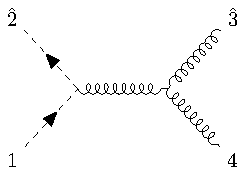
\includegraphics{4pt1.pdf}}
        \end{minipage}
\end{frame}

\begin{frame}
    $\qquad =\raisebox{-2.5em}{\scalebox{0.7}{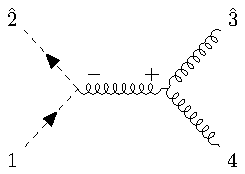
\includegraphics{4pt1.1.pdf}}}+\raisebox{-2.5em}{\scalebox{0.7}{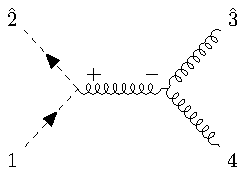
\includegraphics{4pt1.2.pdf}}}$
    \vspace{0.5em}
    
    We denote these two different BCFW channels as $A_1$ and $A_2$, then 
    \begin{align*}
        A_1&=\frac{\avg{\hat{2}\hat{I}}\avg{\hat{I}1}}{\avg{1\hat{I}}}\times \frac{1}{s_{12}}\times \frac{[\hat{I}\hat{3}]^3}{[\hat{3}4][4\hat{I}]}\\
        &=(-1)\frac{\avg{14}^2\avg{24}^2}{\mdavg{12}{23}\!\mdavg{34}{41}}
    \end{align*}
    where we use the fact $\aket{\hat{2}}=\aket{2}$, $\sket{\hat{3}}=\sket{3}$, and the \textcolor{red}{Fierz Identity}
    \begin{equation*}
        [ij][kl]+[il][jk]+[ik][lj]=0
    \end{equation*}
\end{frame}

\begin{frame}
    Similarly, we can obtain
    \begin{equation*}
        A[1,2,3^-,4^+]=(-1)\frac{\avg{13}^2\avg{23}^2}{\mdavg{12}{23}\!\mdavg{34}{41}}
    \end{equation*}
    \textcolor{red}{$\bigstar$ Bonus relation}
    \begin{equation*}
        A[1,2,3^+,4^+]=A[1,2,3^-,4^-]=0
    \end{equation*}
\end{frame}
\begin{frame}
    \frametitle{Fantasitic result from Cauchy Theorem}
    As a result, we can consider amplitude $A_n$ in terms of shifted momentum $\hat{p}_i^\mu$ instead of original real momentum. 
    \begin{equation*}
        A_n \longrightarrow \hat{A}_n(z)
    \end{equation*}
    and we have known the possible positions of single poles, $z_I$, different propagators give 
    us different single poles in the z-plane. 
    \par
    If we consider the meromorphic function $\frac{\hat{A}_n(z)}{z}$ in the complex plane, pick a contour that surrounds the simple pole at the origin. 
    \textcolor{red}{$\bigstar$ The most important point here is that}
    \begin{equation*}
        \boxed{\color{red}\mathrm{Res}|_{z=0}\frac{\hat{A}_n(z)}{z}=\hat{A}_n(0)=A_n}
    \end{equation*}
    It means that the original amplitude equals to the residue at origin.
\end{frame}


\end{document}